\documentclass[a4paper,12pt,twoside,openany]{report}
%
% Wzorzec pracy dyplomowej
% J. Starzynski (jstar@iem.pw.edu.pl) na podstawie pracy dyplomowej
% mgr. inż. Błażeja Wincenciaka
% Wersja 0.1 - 8 października 2016
%
\usepackage{polski}
\usepackage{helvet}
\usepackage[T1]{fontenc}
\usepackage{anyfontsize}
\usepackage[utf8]{inputenc}
\usepackage[pdftex]{graphicx}
\usepackage{tabularx}
\usepackage{array}
\usepackage[polish]{babel}
\usepackage{subfigure}
\usepackage{amsfonts}
\usepackage{verbatim}
\usepackage{indentfirst}
\usepackage[pdftex]{hyperref}
\usepackage{float}
\usepackage{listings}
\usepackage{color}


% rozmaite polecenia pomocnicze
% gdzie rysunki?
\newcommand{\ImgPath}{.}

% oznaczenie rzeczy do zrobienia/poprawienia
\newcommand{\TODO}{\textbf{TODO}}


% wyroznienie slow kluczowych
\newcommand{\tech}{\texttt}

% na oprawe (1.0cm - 0.7cm)*2 = 0.6cm
% na oprawe (1.1cm - 0.7cm)*2 = 0.8cm
%  oddsidemargin lewy margines na nieparzystych stronach
% evensidemargin lewy margines na parzystych stronach
\def\oprawa{1.05cm}
\addtolength{\oddsidemargin}{\oprawa}
\addtolength{\evensidemargin}{-\oprawa}

% table span multirows
\usepackage{multirow}
\usepackage{enumitem}	% enumitem.pdf
\setlist{listparindent=\parindent, parsep=\parskip} % potrzebuje enumitem

%%%%%%%%%%%%%%% Dodatkowe Pakiety %%%%%%%%%%%%%%%%%
\usepackage{prmag2017}   % definiuje komendy opieku,nrindeksu, rodzaj pracy, ...


%%%%%%%%%%%%%%% Strona Tytułowa %%%%%%%%%%%%%%%%%
% To trzeba wypelnic swoimi danymi
\title{Implementacja gry ,,Turbo Slam Dunk Unleashed'' z trybem online multiplayer w środowisku Unity}

% autor
\author{Szymon Piórkowski}
\nrindeksu{279065}

\opiekun{dr hab. inż. Paweł Piotrowski}
%\konsultant{prof. Dzielny Konsultant}  % opcjonalnie
\terminwykonania{25 stycznia 2019} % data na oświadczeniu o samodzielności
\rok{2019}


% Podziekowanie - opcjonalne
\podziekowania{\noindent
{\Large Podziękowania}
\bigskip

Dziękujemy bardzo serdecznie wszystkim, a w szczególności Rodzinom i~Unii Europejskiej...

\bigskip

{\raggedleft
Zdolny Student i Pracowity Kolega

}

}

% To sa domyslne wartosci
% - mozna je zmienic, jesli praca jest pisana gdzie indziej niz w ZETiIS
% - mozna je wyrzucic jesli praca jest pisana w ZETiIS
%\miasto{Warszawa}
%\uczelnia{POLITECHNIKA WARSZAWSKA}
%\wydzial{WYDZIAŁ ELEKTRYCZNY}
\instytut{INSTYTUT ELEKTROENERGETYKI}
\zaklad{ZAKŁAD SIECI I SYSTEMÓW ELEKTROENERGETYCZNYCH}
%\kierunekstudiow{INFORMATYKA}

% domyslnie praca jest inzynierska, ale po odkomentowaniu ponizszej linii zrobi sie magisterska
%\pracamagisterska
%%% koniec od P.W

\opinie{%
  \newpage
\begin{center}
 {\large\bf  Opinia} \\
o pracy dyplomowej magisterskiej wykonanej przez dyplomanta\\
{\bf Zdolnego Studenta i Pracowitego Kolegę} \\
 Wydział Elektryczny, kierunek Informatyka,  Politechnika Warszawska\\
Temat pracy\\
\textit{\bf
TYTUŁ PRACY DYPLOMOWEJ
}\\
\end{center}
\medskip
\noindent
Promotor: {\bf dr inż. Miły Opiekun}\\
Ocena pracy dyplomowej: {\bf bardzo dobry}

\medskip

\centerline{\bf Treść opinii}
   Celem pracy dyplomowej panów dolnego Studenta i Pracowitego Kolegi  było
opracowanie systemu pozwalającego symulować  i opartego o oprogramowanie o
otwartych źródłach (ang. Open Source). Jak piszą Dyplomanci, starali się opracować
system, który łatwo będzie dostosować do zmieniających się dynamicznie wymagań,
będzie miał niewielkie wymagania sprzętowe i umożliwiał dalszą łatwą rozbudowę oraz
dostosowanie go do potrzeb.
Przedstawiona do recenzji praca składa się z krótkiego wstępu jasno i
wyczerpująco opisującego oraz uzasadniającego cel pracy, trzech rozdziałów (2-4)
zawierających opis istniejących podobnych
rozwiązań, komponentów rozpatrywanychjako kandydaci do
tworzonego systemu i wreszcie zagadnień wydajności wirtualnych
rozwiązań. Piąty rozdział to opis przygotowanego przez
Dyplomantów środowiska obejmujący opis konfiguracji
środowiska oraz przykładowe ćwiczenia laboratoryjne. Ostatni
rozdział pracy to opis możliwości dalszego
rozwoju projektu. W ramach przygotowania pracy Dyplomanci zebrali i przedstawili w
bardzo przejrzysty sposób duży zasób informacji, co świadczy o dobrej orientacji
w nowoczesnej i ciągle intensywnie rozwijanej tematyce stanowiącej
zakres pracy i o umiejętności przejrzystego przedstawienia tych
wyników. Praca zawiera dwa dodatki, z których pierwszy obejmuje wyniki
eksperymentów i badań nad wydajnością, a drugi to źródła
skryptów budujących środowisko.

 Dyplomanci dość
dobrze zrealizowali postawione przed nimi zadanie,
wykazali się więc umiejętnością zastosowania w praktyce wiedzy
przedstawionej w rozdziałach 2-4.  Uważam, że cele postawione w założeniach pracy zostały pomyślnie
zrealizowane. Proponuję ocenę bardzo dobrą (5).

\vskip 1cm
{
\raggedleft
(data, podpis)\kern1cm

}
  \newpage
  \newpage
\begin{center}
 {\large\bf  Recenzja } \\
pracy dyplomowej magisterskiej wykonanej przez dyplomanta\\
{\bf Zdolnego Studenta i Pracowitego Kolegę} \\
 Wydział Elektryczny, kierunek Informatyka,  Politechnika Warszawska\\
Temat pracy\\
\textit{\bf
TYTUŁ PRACY DYPLOMOWEJ
}\\
\end{center}
\medskip
\noindent
Recenzent: {\bf prof. nzw. dr hab. inż. Jan Surowy}\\
Ocena pracy dyplomowej: {\bf bardzo dobry}
\medskip


\centerline{\bf Treść recenzji}
   Celem pracy dyplomowej panów dolnego Studenta i Pracowitego Kolegi  było
opracowanie systemu pozwalającego symulować  i opartego o oprogramowanie o
otwartych źródłach (ang. Open Source). Jak piszą Dyplomanci, starali się opracować
system, który łatwo będzie dostosować do zmieniających się dynamicznie wymagań,
będzie miał niewielkie wymagania sprzętowe i umożliwiał dalszą łatwą rozbudowę oraz
dostosowanie go do potrzeb.
Przedstawiona do recenzji praca składa się z krótkiego wstępu jasno i
wyczerpująco opisującego oraz uzasadniającego cel pracy, trzech rozdziałów (2-4)
zawierających bardzo solidny i przejrzysty opis: istniejących podobnych
rozwiązań (rozdz. 2), komponentów rozpatrywanychjako kandydaci do
tworzonego systemu (rozdz. 3) i wreszcie zagadnień wydajności wirtualnych
rozwiązań, zwłaszcza w kontekście współpracy  kilku elementów
 sieci (rozdział 4). Piąty rozdział to opis przygotowanego przez
Dyplomantów środowiska obejmujący opis konfiguracji
środowiska oraz przykładowe ćwiczenia laboratoryjne (5 ćwiczeń). Ostatni, szósty
rozdział pracy to krótkie zakończenie, które wylicza także możliwości dalszego
rozwoju projektu. W ramach przygotowania pracy Dyplomanci zebrali i przedstawili w
bardzo przejrzysty sposób duży zasób informacji o narzędziach, Rozdziały 2, 3 i 4 świadczą o dobrej orientacji
w nowoczesnej i ciągle intensywnie rozwijanej tematyce stanowiącej
zakres pracy i o umiejętności syntetycznego, przejrzystego przedstawienia tych
wyników. Drobne  mankamenty tej części pracy to zbyt skrótowe omawianie
niektórych zagadnień technicznych, zakładające dużą początkową wiedzę czytelnika
i dość niestaranne podejście do powołań na źródła.
Utrudnia to w pewnym stopniu czytanie pracy i zmniejsza jej wartość dydaktyczną
(a ta zdaje się być jednym z celów Autorów), ale jest zrekompensowane zawartością
merytoryczną. Praca zawiera dwa dodatki, z których pierwszy obejmuje wyniki
eksperymentów i badań nad wydajnością, a drugi to źródła
skryptów budujących środowisko. Praca
zawiera niestety dość dużą liczbę drobnych błędów redakcyjnych, ale nie wpływają
one w sposób istotny na na jej czytelność i wartość. W całej pracy przewijają
się samodzielne, zdecydowane wnioski Autorów, które są wynikiem własnych i
oryginalnych badań.  Rozdział 5 i dodatki pracy przekonują mnie, że Dyplomanci dość
dobrze zrealizowali postawione przed nimi zadanie. Pozwala to stwierdzić, że
wykazali się więc także umiejętnością zastosowania w praktyce wiedzy
przedstawionej w rozdziałach 2-4. Kończący pracę rozdział szósty świadczy o
dużym (ale moim zdaniem uzasadnionym) poczuciu własnej wartości i jest
świadectwem własnego, oryginalnego spojrzenia na tematykę przedstawioną w pracy
dyplomowej. Uważam, że cele postawione w założeniach pracy zostały pomyślnie
zrealizowane. Proponuję ocenę bardzo dobrą (5).

\vskip 1cm
{
\raggedleft
(data, podpis)\kern1cm

}
}

\streszczenia{
  \newpage
\begin{center}
\large \bf
Implementacja gry ,,Turbo Slam Dunk Unleashed'' z trybem online multiplayer w środowisku Unity
\end{center}

\section*{Streszczenie}
W ramach pracy dyplomowej zaimplementowano grę komputerową Turbo Slam Dunk Unleashed w środowisku Unity. Projekt został wykonany w języku C\#. Gra została pierwotnie stworzona w środowisku Game Maker Studio, w 2016 roku.
Gra została napisana od początkowi w nowej technologi w celu polepszenia jej jakości oraz zwiększenia możliwości dodawania nowych funkcjonalności. Ponadto została ona rozszerzona o moduł multiplayer, a także wstępnie przygotowana do przeniesienia na nowe platformy (Linux, konsole do gier).

\bigskip
{\noindent\bf Słowa kluczowe:} Unity, C\#, gra komputerowa, grafika komputerowa, Game Maker Studio

\vskip 2cm



\newpage
\begin{center}
\large \bf
Implementation of the game ``Turbo Slam Dunk Unleashed'' in Unity platform, including online multiplayer mode 
\end{center}

\section*{Abstract}
As a part of the diploma thesis, the game Turbo Slam Dunk Unleashed has been implemented in Unity enviroment The proejct has been made using the C\# language. The Game was orginally created in Game Maker Studio enviroment in 2016. Moreover, the game has been extended by online multiplayer module, and pre-prepared to be deployed to new platforms (Linux, game consoles)

\bigskip
{\noindent\bf Keywords:} Unity, C\#, computer game, computer graphics, Game Maker Studio

\vfill
}

\begin{document}
\maketitle

%-----------------
% Wstęp
%-----------------
\chapter{Wstęp}
Celem niniejszej pracy jest przeniesienie gry Turbo Slam Dunk Unleashed do środowiska Unity oraz dodanie do niej modułu online multiplayer. Ponadto, podjęte zostały kroki w celu ułatwienia przygotowania projektu do uruchomienia na nowych platformach. W tym celu gra musiała zostać napisana od zera w języku C\#. Pierwotnie gra została stworzona przez autora niniejszej pracy w środowisku Game Maker.

\section{Gry komputerowe}
Początków gier komputerowych można szukać jeszcze przed pojawieniem się pierwszych komputerów osobistych z interfejsem graficznym. Mało osób wie, że pierwsze gry były produkcjami akademickimi. Takie gry technicznie nie różnią się bardzo od innych programów komputerowych. Są to zwykle programy realizujące zadania takie jak renderowanie, obliczanie logiki gry czy przetwarzanie danych wejściowych od użytkownika w czasie rzeczywistym. Wykorzystywana jest do tego tzw. pętla główna, która jest wykonywana określoną liczbę razy na sekundę. Głównym celem gier jest dostarczenie użytkownikowi rozrywki.

W dzisiejszych czasach gry są niemal wszędzie. Mimo tak krótkiej historii istnieją już klasyki, które zna niemalże każdy gracz. Zdecydowana większość osób młodych miała z już nimi styczność. Popularność gier można zawdzięczać chociażby faktowi, że gry powstają na niemalże każdą platformę elektroniczną - od starszych telefonów komórkowych z dedykowanymi systemami operacyjnymi, po nowoczesne konsole do gier. Do ciekawszych przykładów platform, na które stworzone zostały gry, można zaliczyć: oscyloskopy, czytniki ebooków, zegarki czy telewizory typu SmartTV. Zjawisko to może być porównane do innych dziedzin kultury.

Z punktu widzenia odbiorcy, sam problem stworzenia gry komputerowej może wydawać się pozornie prosty, jednak są to jedne z najbardziej zaawansowanych dzieł ludzkich. Poza kompleksowymi problemami natury programistycznej czy algorytmicznej, dobra gra musi przyciągać uwagę użytkownika i zaspokajać jego ciekawość oraz potrzeby rozrywki. Do osiągnięcia tych celów nierzadko korzysta się z bardzo wielu dziedzin nauki, między innymi: psychologia, fizyka lub biologia.

Ponadto, branża gier komputerowych nie różni się bardzo od branży filmowej czy muzycznej. Powoli zaczyna doganiać ich rozmiar w niektórych krajach, a globalny rynek gier komputerowych przewyższył swoją wartością przemysł filmowy już w 2013 roku. W Polsce z roku na rok branża growa rośnie, a polskie gry są jednym z lepszych towarów eksportowych\cite{canalplus_gry}. Zdecydowanie mają przed sobą ciekawą przyszłość. Dlatego też zagadnienie to jest głównym tematem tej pracy. 

\section{Motywacja}
Pierwotnie Gra Turbo Slam Dunk Unleashed została wykonana w środowisku Game Maker Studio. Środowisko dawało wystarczające możliwości jak na prostotę gry, jednak narzucało również dużo ograniczeń oraz komplikacji. Game Maker jest prostym narzędziem do tworzenia gier dwuwymiarowych. Struktura projektu, którą narzuca to środowisko, sprawia że stosunkowo trudno rozwijać w nim projekty o większej skali. Game Maker korzysta z języka skryptowego Game Maker Language (GML), który składnią przypomina C i Javascript. Skrypty są zwykle krótkimi plikami realizującymi proste zadania. Przez to, naturalnie wraz z wzrostem projektu robi się ich duża ilość, a wyszukiwanie konkretnych zmian staje się coraz trudniejsze. Z tych powodów pisanie warstwy sieciowej wprowadziłoby chaos w wystarczająco skomplikowanym już projekcie.  Ponadto wsparcie dla konsol, mimo swojego istnienia, jest znacznie ograniczone w stosunku do tego w Unity.

Środowisko Unity pozwala pokonać wszystkie te problemy, dodając przy tym projektowi nowego potencjału dla rozwiązywania niektórych, zarówno algorytmicznych, jak i projektowych problemów w grze. Wsparcie samych twórców silnika jest stabilniejsze w przypadku Unity z prostego powodu - komercyjnych gier tworzonych za jego pomocą jest znacznie więcej. Najważniejszym powodem przepisania gry nie była sama technologia, co postęp doświadczenia twórcy. Finalna wersja gry powstała w 2016 roku. Po 3 latach praktyki umiejętności autora znacznie się poprawiły i projekt może zdecydowanie na tym skorzystać. 

\section{Założenia}
Gry komputerowe nie mają jasno określonej granicy ukończenia projektu. Zawsze można coś poprawić, dodać, czy zmienić. W takim projekcie ważne jest, żeby wyznaczyć jasne cele i wymagania, które doprowadzą do stworzenia skończonego produktu. Dlatego też zostały stworzone założenia, które musi spełniać gra, żeby uznać ją za kompletną:

\begin{itemize}
    \item Przeniesienie gry w wersji podstawowej do środowiska Unity
    \begin{itemize}
        \item Mecz 2 graczy na 1 komputerze,
        \item Rzucanie i zabieranie piłki, faule,
        \item Liczenie punktów, stan meczu,
        \item Wybór postaci, piłki, planszy oraz czasu meczu.
    \end{itemize}
    
    \item Dodanie trybu online multiplayer
    \begin{itemize}
        \item Mecz 2 graczy na 2 komputerach przez sieć,
        \item Synchronizacja pozycji graczy oraz piłki,
        \item Synchronizacja stanu meczu - punkty, faule, czas,
        \item Synchronizacja wyboru ustawień meczu - wygląd graczy, piłki, mapa oraz czas meczu,
        \item Możliwość dołączenia do losowego gracza lub gry ze znajomym,
        \item Obsługa błędów związana z problemami z połączeniem.
    \end{itemize}
    
    \item Przygotowanie gry do przeniesienia na nowe platformy
    \begin{itemize}
        \item Przygotowanie warstwy abstrakcji wejść,
        \item Optymalizacja logiki i warstwy sieciowej.
    \end{itemize}
\end{itemize}



%-----------------
% Opis Środowiska
%-----------------
\chapter{Opis Środowiska}
W tym rozdziale znajduje się opis narzędzi, przy pomocy których został zrealizowany projekt gry.
\section{Unity}
Unity jest częściowo darmowym silnikiem do tworzenia gier, stworzonym w 2005 roku. Od tego czasu silnik był wielokrotnie modyfikowany i zostało opublikowane wiele nowych wersji. Obecnie najnowsza stabilna wersja oznaczona jest numerem 2018.3\cite{unity_wiki}. Silnikiem do gry nazywamy zestaw narzędzi, oraz sprawdzonych algorytmów, które często używane są do tworzenia gier. Pierwsza wersja Unity została stworzona przez 3 kolegów - Davida Helgason, Joachima Ante oraz Nicholasa Francisa w Danii. Unity posiada kilka typów licencji. Podstawowa z nich jest darmowa, jednak po przekroczeniu określonego przez Unity pułapu przychodów, należy kupić licencję wyższego poziomu. Płatne licencje nie dają tylko takiej możliwości, rozszerzają one nieco możliwości edytora a także zwiększają wsparcie twórców gier. W przypadku najdroższej wersji - Enterprise, użytkownicy silnika mają nawet dostęp do kodu źródłowego silnika.

\begin{table}[h!]
\centering
\begin{tabular}{c|cccc}
Nazwa Wersji & Limit przychodów & Wsparcie premium & Cena \\ \hline
Personal & \$100,000 & NIE & Darmowa \\
Plus & \$200,000 & NIE & \$420 rocznie \\
Pro & Nielimitowane & TAK & \$1500 rocznie \\
Enterprise & Nielimitowane & TAK & Indywidualnie \\
\end{tabular}
\caption{Zestawienie licencji Unity (źródło: \cite{unity_wiki})}
\label{table_unity_versions}
\end{table}

\begin{figure}[!htbp]
	\begin{center}
\centering
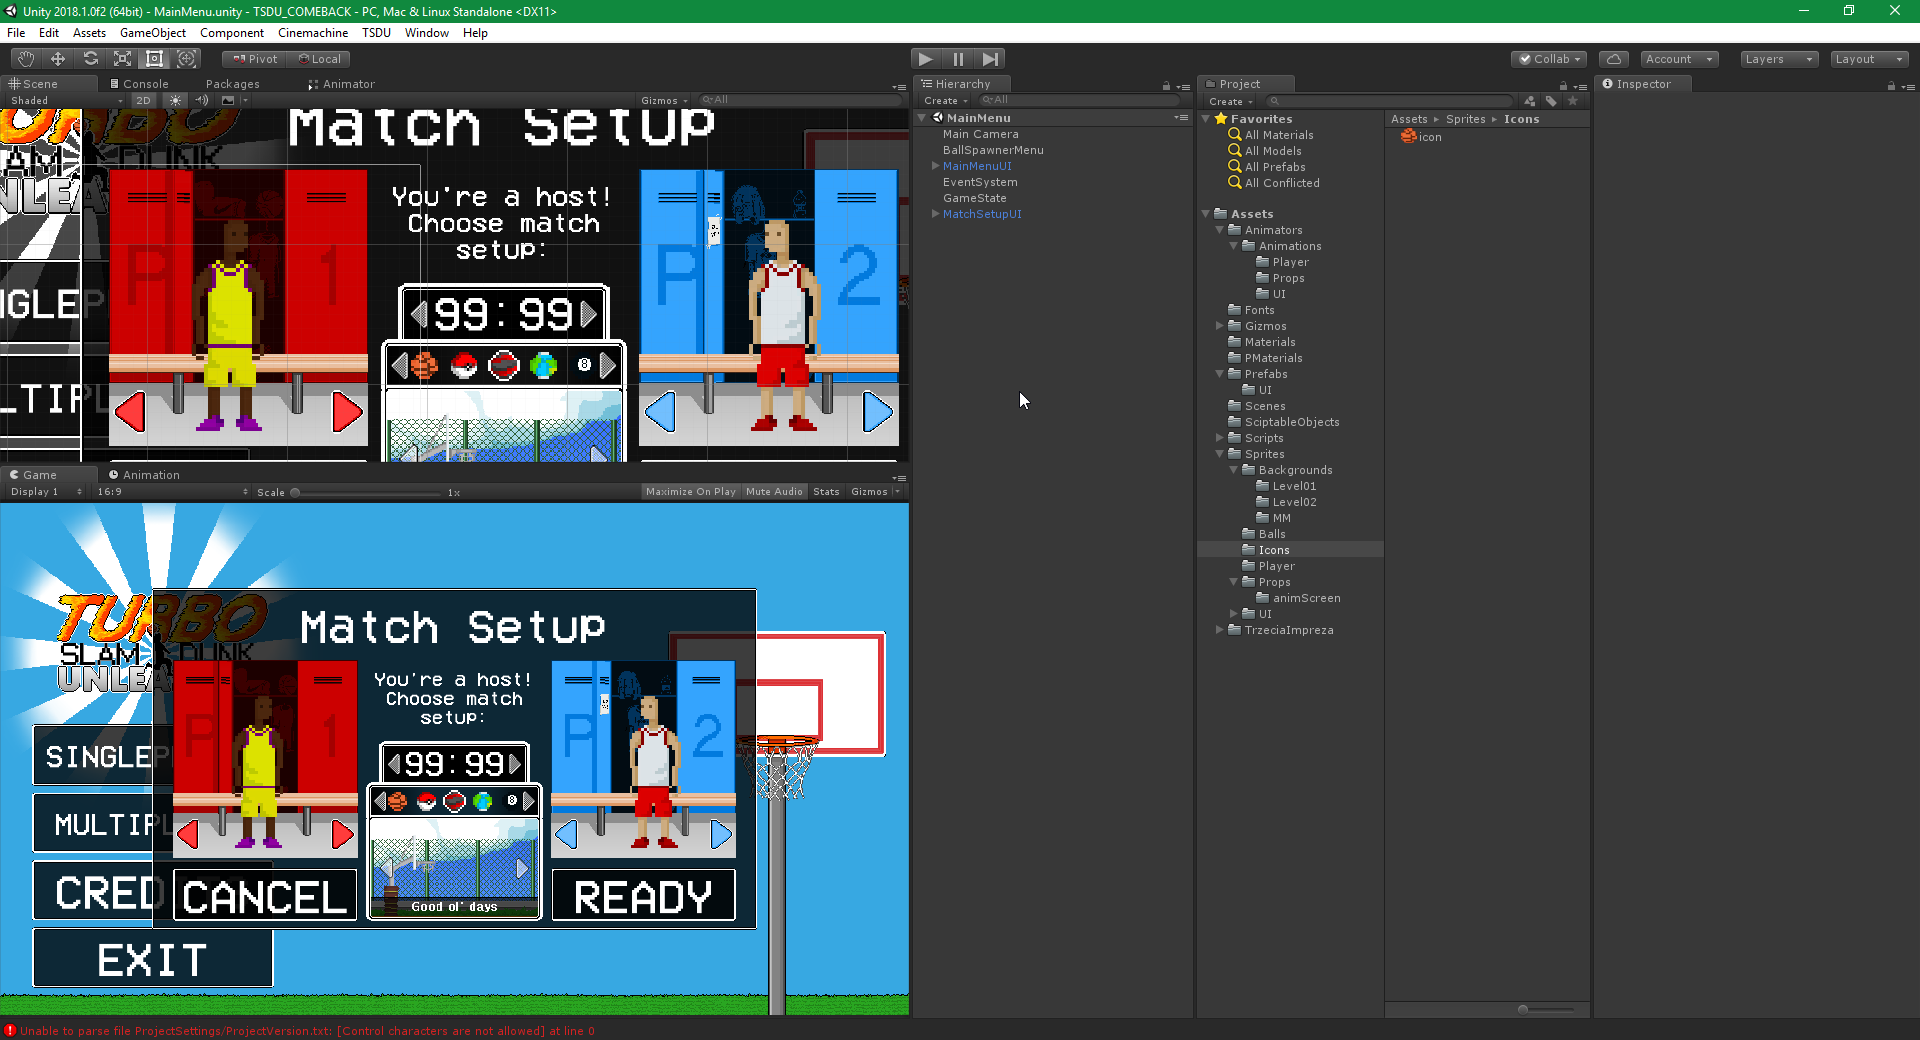
\includegraphics[scale=0.2]{\ImgPath/rys/unity_home.png}
\end{center}
	\caption{Domyślny widok edytora Unity w projekcie gry}
	\label{unity_home}
\end{figure}

Na chwilę obecną silnik obsługuje 27 platform: iOS, Android, Tizen, Windows, Universal Windows Platform, macOS, Linux, WebGL, PlayStation 4, PlayStation Vita, Xbox One, Wii U, 3DS, Oculus Rift, Google Cardboard, SteamVR, PlayStation VR, Gear VR, Windows Mixed Reality, Daydream, Android TV, Samsung Smart TV, tvOS, Nintendo Switch, Fire OS, Facebook Gameroom, Apple's ARKit, Google's ARCore, and Vuforia. Jest to dość długa lista jak na silnik do tworzenia gier. Zwykle ograniczają się one do mniejszej liczby platform. Dlatego też gra stworzona w tym silniku ma bardzo duży potencjał do zaistnienia na większej ilości platform, a co za tym idzie - zyskanie nowych graczy. Samo przeniesienie między platformą jest reklamowane przez Unity jako bardzo prosta akcja - wystarczy jeden przycisk. W praktyce jednak zależy to bardzo od typu gry oraz tego jak wygląda architektura samej gry.

Silnik napisany jest w językach C, C++ oraz C\#. W pierwszych dwóch napisane są podstawy silnika takie jak renderowanie, logika czy obsługa wejść. Trzeci z tych języków został użyty do napisania warstwy wizualnej - GUI edytora oraz do stworzenia podstawowych komponentów. Może on być również używany przez twórców gier do tworzenia własnych komponentów lub rozszerzeń silnika. Unity przyjmuje podejście komponentowe. Typ obiektu w grze jest definiowany przez zestaw jego komponentów. Komponenty są mniejszymi elementami, które realizują określone zdania. Do podstawowych typów komponentów można zaliczyć między innymi:
\begin{itemize}
    \item \textit{Transform} - Posiada go każdy GameObject, służy do określenia pozycji, rotacji oraz skali obiektu w przestrzeni trójwymiarowej sceny. Transformy tworzą hierarchię sceny podobną do drzewa. Dzięki temu można np. tworzyć skompilowane obiekty na scenie, a następnie poruszać je całe poprzez translację jednego, nadrzędnego transforma.
    \item \textit{Camera} - Podstawa renderingu, wyświetla na danym ekranie część sceny, którą aktualnie obejmuje. Posiada 2 tryby projekcji - ortogonalną oraz perspektywiczną. Z zasady pierwszy typ wykorzystywany jest dla gier dwuwymiarowych, natomiast drugi dla trójwymiarowych.
    \item \textit{Sprite Renderer} - Komponent odpowiedzialny za rysowanie dwuwymiarowych grafik - tzw. Sprite'ów. Posiada różne tryby rysowania, obroty w osiach X i Y, kolejność sortowania oraz możliwość przemnożenia kolorów obrazka przez jeden wybrany kolor.
    \item \textit{Box Collider 2D} - Komponent ten umożliwia rejestrowanie kolizji - fundamentalnej funkcjonalności gry. Kolizje występują kiedy dwa obiekty są w kontakcie, a także dostarczają szczegółowych informacji o tych kontaktach. Typ Box jest prostszym kształtem, istnieją też inne bardziej lub mniej skomplikowane kształty colliderów.
    \item \textit{Rigidbody 2D} - Podstawa symulacji fizyki dwuwymiarowej w Unity. Obiekt posiadający ten komponent musi również posiadać komponent typu Collider 2D, żeby móc odbierać informacje o kolizjach. Posiada zestaw zmiennych umożliwiających symulację fizyki: masa, pozycja, prędkość, prędkość kątowa oraz środek ciężkości. Ulega też grawitacji, jeżeli taka jest zdefiniowana na scenie.
    \item \textit{Animator} - Odpowiada za animacje niemalże dowolnej wartości obiektu. Poprzez animację można rozumieć zmianę wartości w czasie. Najczęściej służy do zmiany pozycji obiektów, ale można nim także zmieniać pojedyncze zmienne komponentów, takie jak kolor czy sprite. Animator jest realizowany w postaci maszyny stanów.
    \item \textit{Canvas} - Podstawa interfejsu użytkownika. Definiuje przestrzeń, w której wyświetlane są jego elementy. Może być ona wyświetlana jako narzuta na okno gry, narzuta na konkretną kamerę, lub płaszczyzna w przestrzeni trójwymiarowej.
    \item \textit{Mono Behaviour} - Komponenty tego typu są skryptami w języku C\#. Można więc swobodnie je definiować i stworzyć w nich niemalże dowolną funkcjonalność. Więcej informacji o skryptowaniu znajduje się w sekcji ,,Język C\# oraz Mono''.
\end{itemize}
Powyższe elementy są najczęściej wykorzystywane podczas tworzenia gry dwuwymiarowej. Istnieje szereg komponentów o funkcjonalności trójwymiarowej, ale jako że gra opisywana w tej pracy operuje tylko na dwóch wymiarach, zostały one pominięte.

\section{Język C\# oraz Mono}

Do programowania rozgrywki oraz logiki gry używa się języka C\#. Nie jest on jednak natywnym językiem silnika. Żeby możliwe było obsługiwanie skryptów w tym języku, Unity używa zewnętrznej platformy zwaną Mono. Mono jest open-sourcowym projektem opartym na frameworku .Net\cite{about_mono}. Pozwala między innymi na łatwe budowanie aplikacji na wiele platform.

\begin{figure}[!htbp]
	\begin{center}
\centering
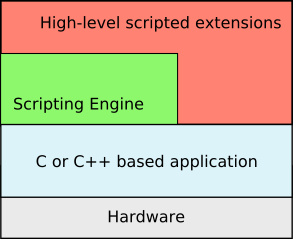
\includegraphics[scale=0.6]{\ImgPath/rys/mono_architecture_scripting.png}
\end{center}
	\caption{Architektura implementacji C\# jako język skryptowy w Mono}
	\label{mono_architecture_scripting}
\end{figure}

W przeszłości do podobnych celów wykorzystywało się języki skryptowe. Wiele silników posiadało własne mniej lub bardziej wydajne implementacje. Często jednak wielkość skryptów przekraczała możliwości interpretatora lub nawet silnika skryptowania, przez co możliwości były bardzo ograniczone. Mono używa różnych języków do różnych celów, a więc traktuje je jako narzędzia, które służą do rozwiązywania innych problemów.

Podczas gdy ważna, krytyczna część aplikacji może być napisana w wydajnym nisko poziomowym języku jak C, częściami takimi jak interfejs użytkownika czy interakcje z użytkownikiem zajmuje się język wyższego poziomu, który nie jest tak samo wydajny, ale pozwala zmniejszyć ilość wymaganych linijek kodu do zrealizowania konkretnego zadania. Kod napisany w takim języku jest zdecydowanie wolniejszy od kodu natywnego, ale w porównaniu z popularnymi językami skryptowymi takimi jak np. LUA jest zdecydowanie szybszy. Mono umożliwia bardzo proste wołanie metod w języku natywnym, przez co łatwo jest podzielić zadania na te, które powinny być napisane optymalnie, oraz na te, które nie wymagają aż takiej oszczędności. Wspierane jest wiele języków wyższego poziomu, do których należą miedzy innymi: C\#, Java, F\#, Python czy JavaScript.

Język C\# jest stworzonym dla Microsoft obiektowym językiem programowania. Kod napisany w tym języku kompilowany jest do Common Intermediate Language (CIL), który jest z kolei wykonywany w środowisku uruchomieniowym  takim jak .Net czy właśnie Mono.  


\begin{figure}[!htbp]
	\begin{center}
\centering
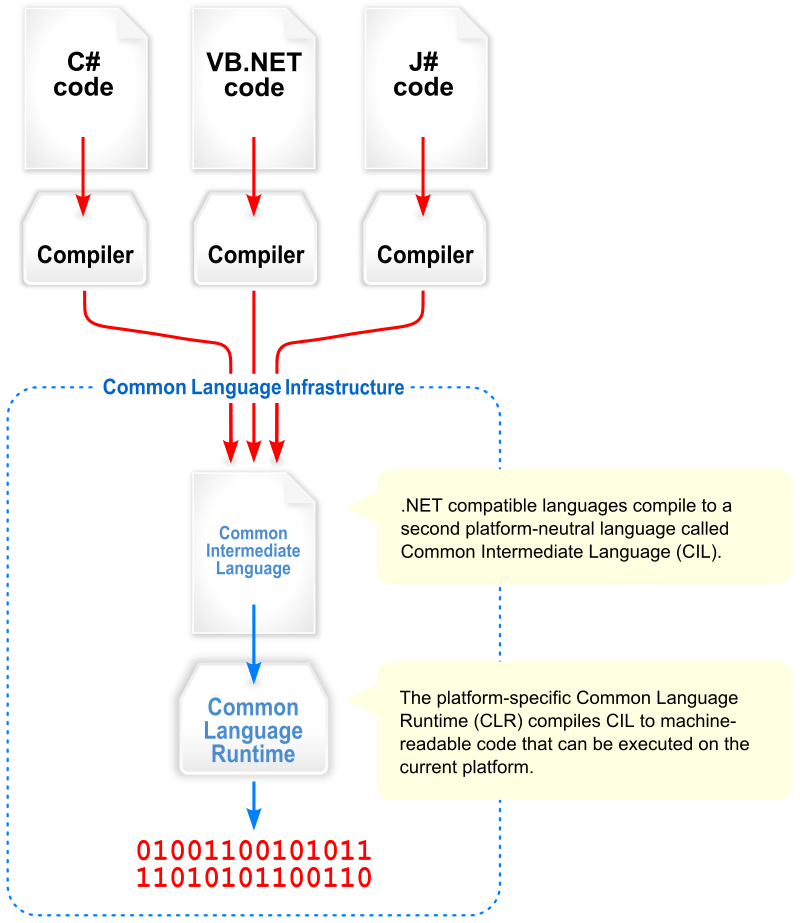
\includegraphics[scale=0.43]{\ImgPath/rys/CIL.png}
\end{center}
	\caption{Schemat pokazujący proces kompilacji języka wykorzystującego CIL}
	\label{CIL}
\end{figure}

Język ten jest silnie typowany, deklaratywny, imperatywny oraz funkcyjny. Powstał w około 2000 roku i został zaakceptowany jako standard przez ECMA (ECMA-334) oraz ISO (ISO/IEC 23270:2006). Posiada wiele przydatnych funkcji:
\begin{itemize}
    \item Odśmiecanie pamięci - C\# automatycznie zarządza pamięcią poprzez liczenie referencji do obiektów. Jeżeli do danego obiektu nie prowadzi żadna referencja, jest on niszczony podczas przebiegu tzw. Garbage collectora.
    \item Delegaty oraz Zdarzenia - bardzo wygodny sposób na kontrolowanie wykonywania kodu i uruchomienie go podczas zdarzeń. Jest to pewnym rozszerzeniem wskaźników, które możemy spotkać w językach niższego poziomu.
    \item Refleksja i atrybuty klas - Podczas działania programu istnieje możliwość analizy jego struktury z poziomu tego kodu. Przydaje się chociażby podczas debugowania kodu czy innych zastosowaniach, które korzystają z nieznanej podczas kompilacji struktury kodu.
    \item Typy generyczne - mechanizm zbliżony do działania szablonów w C++. Pozwala na tworzenie całych klas operujących na danych o nieznanym typie, ale posiadającym konkretny zestaw funkcji.
\end{itemize}

\section{Dodatkowe narzędzia}
Do stworzenia kompletnej gry teoretycznie wystarczy sam silnik, jednak używanie zewnętrznych programów do tworzenia plików znacznie poprawia jakość zarówno samej produkcji, jak i pracy nad nią. Poniżej znajduje się lista użytego oprogramowania:

\begin{itemize}
    \item Microsoft Visual Studio 2017 - środowisko programistyczne wspierające wiele języków. Możliwe jest doinstalowanie pakietu integracji z Unity. Poza edycją skryptów pozwala na debugowanie projektu poprzez wbudowany debugger.
    \item Git - Darmowy i open soure'cowy program służący do kontroli wersji. Jest to program konsolowy. Bardzo przydaje się do śledzenia zmian, a także do łatwego tworzenia kopii zapasowej plików projektowych.
    \item Git Extensions - Darmowy i open source'owy program do obsługi gita. Uzupełnia gita o graficzny interfejs, co ułatwia pracę przy dużych projektach. Zamyka też wiele skomplikowanych komend w przystępne guziki, co uprzyjemnia pracę z gitem.
    \item Paint.Net - Darmowy i open sourcowy program do edycji grafiki. Napisany w języku C\# z wykorzystaniem frameworku .Net. Bardzo prosty w obsłudze program, dzięki któremu poprawki grafiki zostały wykonane szybko i precyzyjnie bez utraty jakości.
    \item TexturePacker - Program do pakowania grafik w tzw. atlasy. Taki sposób przechowywania grafik umożliwia prostsze animowanie, jest wydajniejszy pamięciowo oraz pozwala ominąć kilka innych problemów związanych z importowaniem dużej ilości grafik do projektu z grą.
\end{itemize}

%-----------------
% Opis gry “Turbo Slam Dunk Unleashed”
%-----------------
\chapter{Opis gry ,,Turbo Slam Dunk Unleashed''}

\section{Historia}

Proces tworzenia gry rozpoczął się w 2015 roku, a jej pełna wersja została udostępniona w serwisie Gamejolt.com 3 czerwca 2016 roku\cite{gamejolt_page}. Na początku był to projekt hobbystyczny, który potem zamienił się w projekt kołowy i był tworzony w ramach Koła Naukowego Twórców Gier "Polygon". Finalna wersja została zaprezentowana na jednym z pokazów projektów kołowych.
\begin{figure}[!htbp]
	\begin{center}
\centering
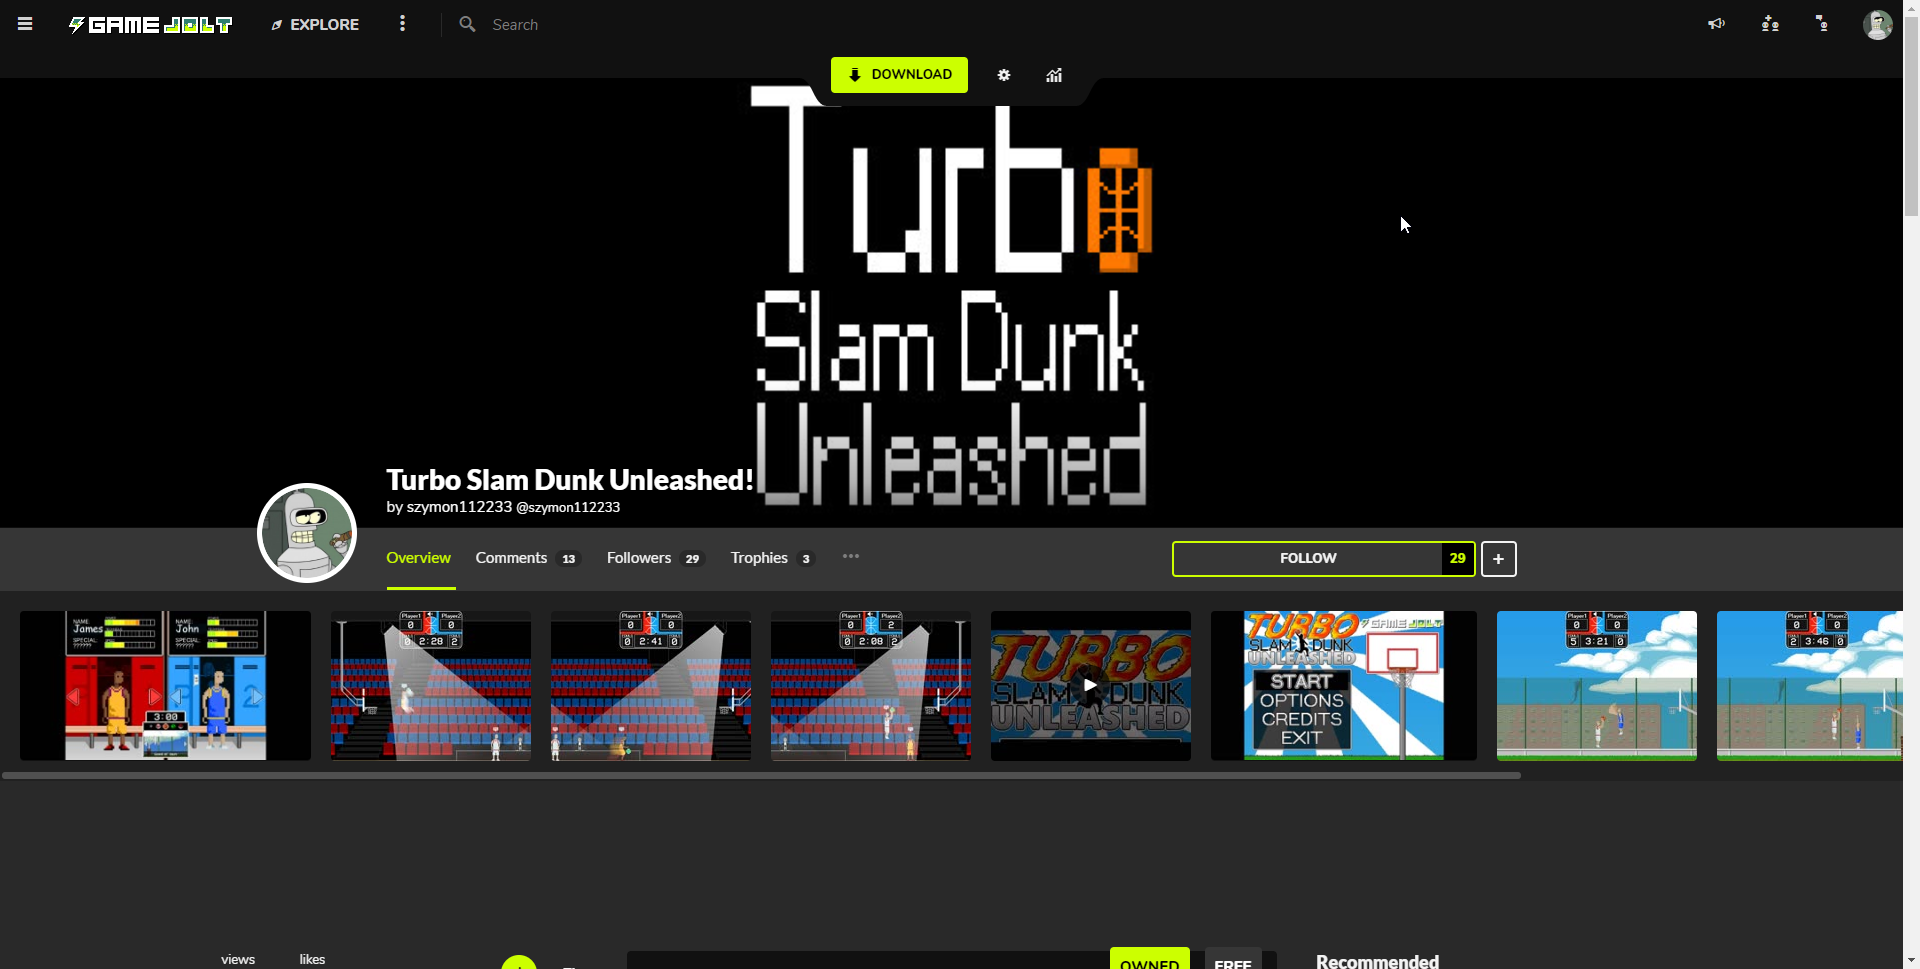
\includegraphics[scale=0.25]{\ImgPath/rys/gamejolt_page.png}
\end{center}
	\caption{Strona główna gry w serwise Gamejolt.com}
	\label{gamejolt_page}
\end{figure}

\section{Ogólny opis gry}
Głównym elementem rozgrywki są mecze koszykówki miedzy dwoma graczami rywalizującymi na jednym komputerze. Gracze używają jednej klawiatury lub padów żeby poruszać swoimi postaciami w świecie gry. Istnieje jedna piłka, której wrzucenie do kosza przeciwnika powoduje zdobycie punktu. W grze istnieją również faule. Faul to sytuacja gdy jeden gracz uderzy drugiego żeby zabrać mu piłkę  w które gracz wyskoczył z piłką i jej nie rzucił - tak jak w prawdziwej koszykówce. Faule są liczone i odejmowane od zdobytych punktów pod koniec meczu. Mecz trwa określony czas, domyślenie 3 minuty i po tym czasie liczone są punkty i wyświetlany jest werdykt meczu.

\section{Opis elementów gry}

Gra jest bardzo prosta i składa się z kilku podstawowych elementów.
Poniżej znajduje się obrazek pokazujący graficzne reprezentacje wymienionych elementów.
\begin{enumerate}
    \item Plansza - Świat gry w którym poruszają się gracze, głównie są to elementy wizualne
    \item Postacie graczy - W grze istnieją 2 instancje. Jest ona sterowana przez człowiek poprzez zestaw wejść. Może chodzić w lewo lub w prawo, skakać, rzucać piłkę oraz uderzać. Dwie ostatnie akcje możliwe są zarówno podczas stania jak i w locie. Skok służy do zwiększenia zasięgu rzutu lub po prostu lepszego do niego ustawienia. Obrót gracza jest niemożliwy w powietrzu, pozwala to na dokładniejsze dostosowanie swojej pozycji do rzutu. Rzut piłki służy głownie do umiejscowienia jej w obręczy kosza. Po rozpoczęciu przyciskania klawisza odpowiedzialnego za rzut, gracz traci możliwość chodzenia i jest w trakcie rzutu. Podczas tego czasu pokazuje się wskaźnik siły rzutu który oscyluje między minimalną i maksymalna siłą rzutu. Po puszczeniu przycisku piłka jest rzucana zgodnie z siłą która była wskazana w tym momencie. Uderzanie służy do zabierania piłki drugiemu graczowi. Po przyciśnięciu klawisza uderzenia rozpoczyna się animacja uderzenia i jeżeli trafiliśmy ręką w punkt w którym znajduje się piłka piłka jest wybijana drugiem graczowi. W trakcie trwania animacji, możliwość chodzenia jest zablokowana.
    \item Piłka - Główny element, służy do zdobywania punktów przez graczów. Jej fizyka jest symulowana w 2 wymiarach, przez co uzyskujemy bardzo ciekawe efekty jej wyrzutu. Jeżeli znajdzie się w obręczy kosza, naliczane są 2 punkty graczowi atakującemu ten kosz. Jeżeli piłka została wyrzucona z odpowiednio dużej odległości, trafienie daje dodatkowy punkt. Jeżeli piłka wyleci poza boisko to jej pozycja resetuje się do środka planszy, a gracze pojawiają się na swoich początkowych pozycjach.
    \item Kosze -  W grze istnieją 2 instancje. Trafienie do jednego z nich dodaje punkty. Ich wygląd różni się zależnie od planszy, ale sama funkcjonalność pozostaje niezmienna.
    \item Tablica Wyników - Pokazuje aktualny stan meczu - pozostały czas, ilość punktów oraz ilość fauli każdego z graczy. na środku tablicy znajduje się grafika piłki, której kolor zmiana się zależnie od wyniku meczu.
\end{enumerate}

\begin{figure}[!htbp]
	\begin{center}
\centering
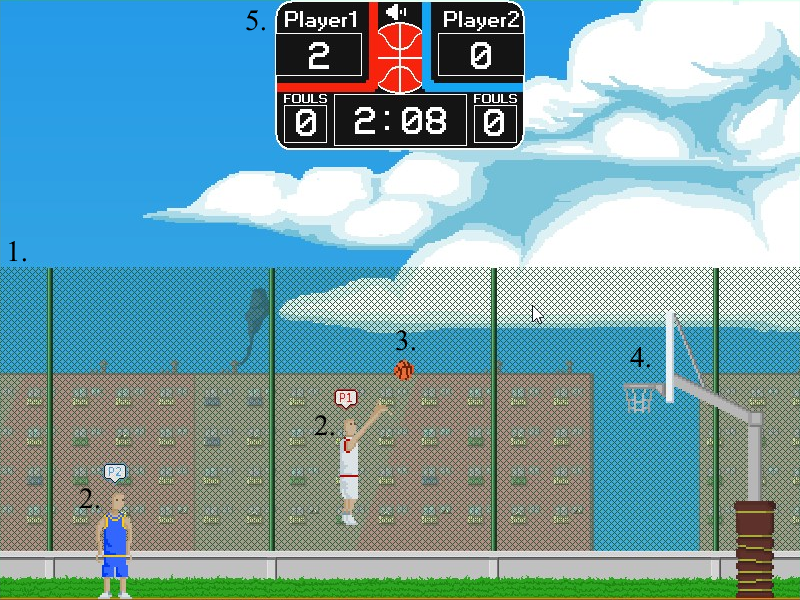
\includegraphics[scale=0.6]{\ImgPath/rys/game_elements.png}
\end{center}
	\caption{Elementy gry na zrzucie ekranu z aplikacji}
	\label{game_elements}
\end{figure}

\section{Inne funkcjonalności}
Wyżej wymienione elementy stanowią podstawę gry. Teoretycznie wystarczą one do przeprowadzenia pełnej rozgrywki jednak, nie wydaje się ona zbyt ciekawa. Gra posiada wiele funkcjonalności które ułatwiają rozgrywkę, zwiększają jej komfort, bądź też jej odczucie przez gracza:
\begin{itemize}
    \item Ekran ustawień - pozwala na ustawienie klawiszy które odpowiedzialne są za konkretne akcje w grze, oraz ustawienie poziomu głośności dźwięków. Ustawienia te są zapisywane w pliku .ini przez co po restarcie gry nie trzeba ich od nowa ustawiać. 
    \item Ekran ustawień meczu - pozwala na zmianę ustawień pojedynczego meczu. Zmienione może zostać:
    \begin{itemize}
        \item Czas meczu
        \item Wygląd postaci każdego z graczy
        \item Wygląd piłki
        \item Plansza
    \end{itemize}
    \item Dźwięki - zwiększają immersję i stanowią dodatkową informacje zwrotną z gry. W grze można usłyszeć dźwięki tła z plansz, uderzeń piłki o różne powierzchnie, gwizdka sygnalizujące faul, oraz dźwięki wyboru przycisku w menu.
    \item Efekty cząsteczkowe - Małe dodatki graficzne które sprawiają że gra wygląda ciekawiej. Można do nich zaliczyć efekt sypiącego się piasku gdy postać rusza. 
    \item Efekty specjalne - Głównie lekkie trzęsienie kamerą przy uderzeniach piłki o kosz. Stanowią dodatkową informacje zwrotną z gry.
    \item Dynamiczna kamera - Kamera która zawsze pokazuje w kadrze piłkę lub gracza z piłką. Gracz z piłką nie jest na środku, ponieważ kamera pokazuje zdecydowanie więcej strony w którą jest aktualnie zwrócony, tak żeby można było swobodnie rzucać.
    \item Obsługa padów - Gracze mogą nie chcieć używać klawiatury do gry z wielu powodów, dlatego też gra w pełni wspiera obsługiwanie jej tzw. padem czyli specjalnym kontrolerem stworzonym właśnie do grania w gry. Dzięki temu każdy gracz może wybrać swój preferowany sposób obsługi i nie musi dzielić klawiatury z przeciwnikiem.
    \item Osiągnięcia - Strona Gamejolt.com posiada system osiągnięć. Każdy użytkownik może je odblokować jeżeli zostały one zaimplementowane przez developera. W grze istnieją 3 osiągnięcia. Osiągnięcia są często ciekawym dodatkiem do gry i przedłużają czas jaki można spędzić                 nad grą.
    \item Znaczniki pozycji - Ponieważ postacie graczy nie zawsze są w kadrze, gracze nie posiadają informacji o swojej pozycji. Dzięki prostym strzałkom w kolorze gracza ta informacja jest zachowana. Ponadto, ponieważ możliwa jest zmiana wyglądu kontrolowanej postaci, a nawet możliwy jest wybór takiego samego wyglądu dla obu graczy, nad ich głowami widnieją znaczniki z numerem gracza.
\end{itemize}


\begin{figure}[!htbp]
	\begin{center}
\centering
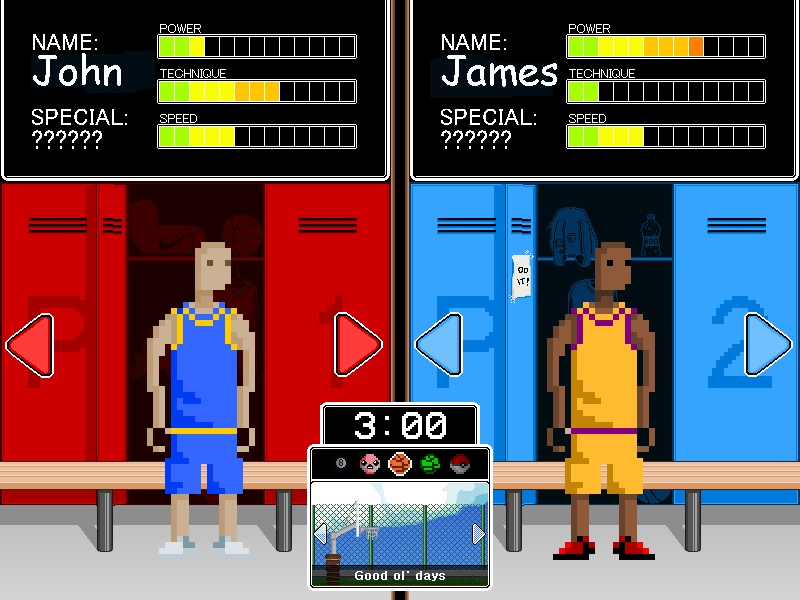
\includegraphics[scale=0.5]{\ImgPath/rys/match_setup_old.png}
\end{center}
	\caption{Ekran ustawień meczu}
	\label{match_setup_old}
\end{figure}


%-----------------
% Implementacja
%-----------------
\chapter{Implementacja nowej wersji gry}

Tak jak zostało już wspomniane wcześniej, gra została przepisana od zera w środowisku Unity. W tym rozdziale znajduje się szczegółowy opis implementacji.

\section{Zmiany w stosunku do oryginalnej wersji gry}

Oryginalnej gra była atrakcyjna dla graczy, jednak z perspektywy czasu jej design może być poprawiony w wielu aspektach. Niektóre aspekty okazały się nietrafione a inne po prostu mogą być ulepszone o nowe pomysły. W obecnej wersji zostały wprowadzone następujące zmiany w stosunku do wersji oryginalnej:
\begin{itemize}
    \item Dodanie trybu online multiplayer - W oryginalnej grze możliwa była tylko gra na jednym komputerze. Dlatego też niezbędna była obecność 2 graczy przy jednym urządzeniu. Dzięki wprowadzeniu takiego trybu, gracze nie muszą być teraz fizycznie w jednym miejscu. Nie muszą też współdzielić klawiatury.
    \item Zmiana rozmiaru okna gry - Oryginalna gra jest wyświetlana w oknie o rozdzielczości 800x600. Jest to zdecydowanie przestarzała rozdzielczość nie mówiąc już o jej współczynniku proporcji - 4:3. Użytkownicy posiadają monitory o wile większych rozdzielczościach najczęściej w 16:9. Dlatego też gra zaczęła wspierać rozdzielczość 1920x1080  nazywaną czasami FullHD jako domyślną. Większość monitorów komputerów PC operuje na takiej rozdzielczości lub innych o takim samym współczynniku proporcji. Tak długo jak jest on zachowany okno gry skaluje się poprawnie i widoczne są wszystkie elementy gry.
    \item Poprawa kamery - Kamera nie różni się bardzo od podstawowej wersji, jednak zostały wprowadzone małe usprawnienia. Śledzony jest teraz każdy gracz oraz piłka, zamiast tylko gracza z piłką lub samej piłki. Dzięki temu kluczowe elementy gry zawsze znajdują się w polu widzenia. Przed każdym graczem widoczna jest też konkretna przestrzeń, tak żeby kosze były widoczne. Dzięki takiemu rozwiązaniu możliwe jest też zobaczenie całej mapy na ekranie.  
    \item Zmiana systemu kolorowania graczy - W wersji oryginalnej warianty kolorystyczne graczy były realizowane poprzez podmianę spritów gracza. W takim rozwiązaniu dla każdego wariantu kolorystycznego musiał powstać zestaw wszystkich klatek animacji. W wersji obecnej zmiana koloru odbywa się w tzw. shaderze. Jest to część kodu wykonywana na karcie graficznej podczas rednerowania. Shader korzystając z maski zamienia kolory gracza w każdej animacji, przez co możliwe jest stworzenie niemalże nieskończonej liczby wariantów, bardzo tanim kosztem. Rozwiązanie te jest też dużo wydajniejsze pamięciowo - każdy nowy wariant nie wymaga tworzenia plików które ładowane są do pamięci.
    \item Zmiany zasad rozgrywki - W wersji oryginalnej wyrzucenie piłki poza plansze oznaczało restart pozycji graczy oraz piłki za każdym razem. W tej wersji piłka jest po prostu odrzucana ze strony z której wyleciała. Pozwala to zachować dynamikę gry i jest nieco humorystycznym akcentem w grze. Ponadto zdobycie punktów, po prostu resetuje pozycję graczy zamiast ustawiać ich w pozycji zależenie od tego kto zdobył punkt i jaki kosz został zaatakowany.
    \item Usunięcie achievementów - W oryginalnej wersji nie ciszyły się zbytnią popularnością. Były też związane bezpośrednio z serwisem Gamejolt.org na którym nowa wersja nie będzie dostępna. Możliwe jednak że zostaną one dodane w przyszłości dla innych platform.
    \item Usunięcie znaczników pozycji - Z powodu zmian w kamerze, postacie zawsze widoczne są na ekranie. Nie ma więc potrzeby stosowania znaczników, tak jak było to zrobione w poprzedniej wersji gry.  
    \item Usuniecie obsługi padów - Ponieważ system wejść został napisany od zera, praca nad nim zajęła dużo czasu. Zrobienie dobrej obsługi innych kontrolerów niż standardowa klawiatura nie jest trywialnym zadaniem zwłaszcza jeżeli chodzi o nawigowanie po interfejsie użytkownika. Zadanie to jednak musi zostać zrealizowane jeżeli gra miałaby ukazać się na konsolach do gier.
    \item Brak mniejszych szczegółów - W oryginalnej wersji istnieje dużo drobnych szczegółów, których nie widać na pierwszy rzut oka. Sprawiają one że gra wydaje się bardziej kompletna. Można do nich zaliczyć efekty cząsteczkowe, specjalne czy dźwiękowe. Praca nad takimi szczegółami jest bardzo czasochłonna, a granie jest możliwe bez nich, dlatego też ich implementacja została odłożona na późniejszy czas.
\end{itemize}

\section{Implementacja gry z wykorzystaniem środowiska Unity}
Główną sceną gry jest scena o nazwie "Main Menu". Jej głównym celem jest umożliwienie graczowi nawigacji po grze. Jest też ona pierwszą rzeczą jaką gracz zobaczy w grze dlatego ważne jest żeby była ciekawa. Po lewej stronie znajduje się panel przycisków, a nad nimi umiejscowione jest logo gry wraz z prostą animacją. W tle widać też spadające piłki koszykowe.

\begin{figure}[!htbp]
	\begin{center}
\centering
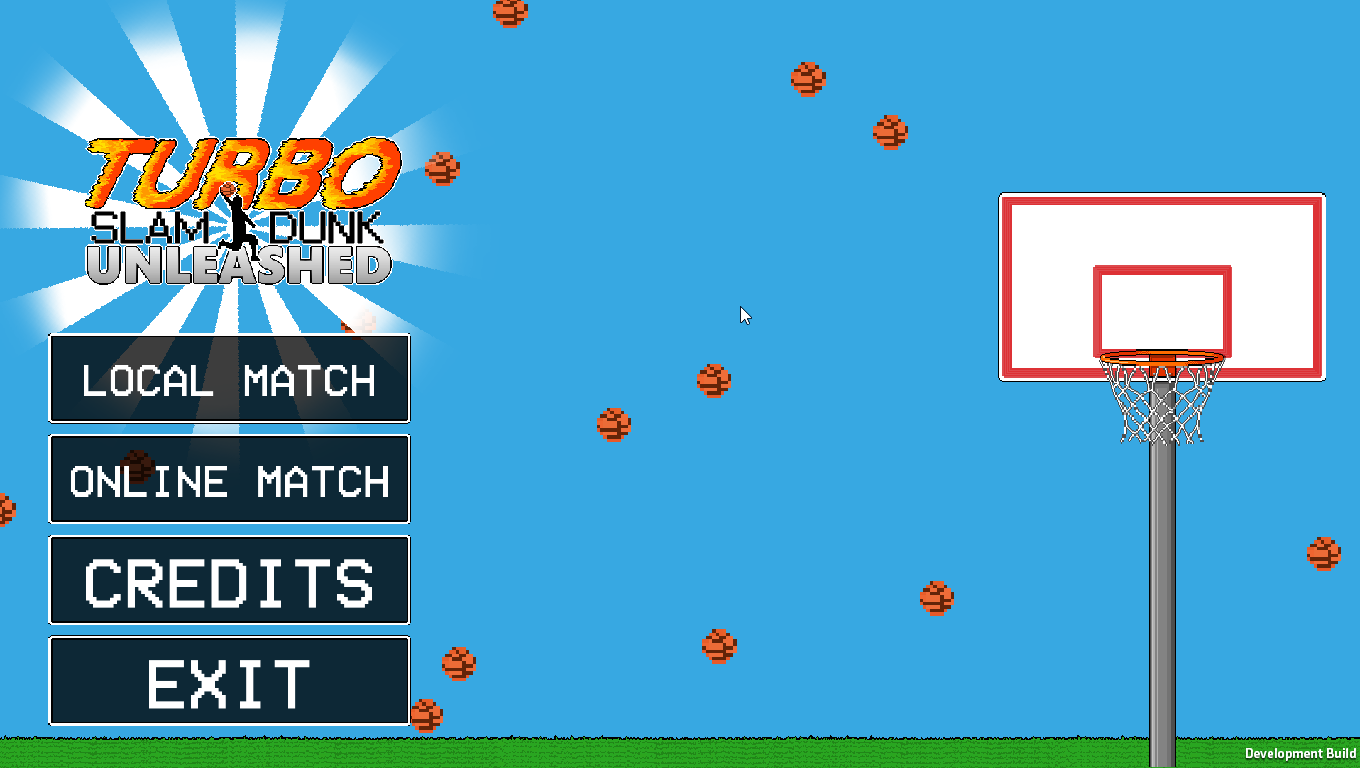
\includegraphics[scale=0.3]{\ImgPath/rys/main_menu.png}
\end{center}
	\caption{Ekran głównego menu}
	\label{main_menu}
\end{figure}

Zdecydowana większość sceny jest interfejsem użytkownika. Dlatego też znajduje nadrzędnym elementem sceny jest obiekt \textit{MainMenuUI}. Posiada on komponent Canvas oraz wszystkie wymagane przez niego komponenty czyli CanvasScaler oraz Graphics Raycaster. Posiada również Mono Behaviour "MainMenuUI"  który odpowiada za całą jego logikę którego kod znajduje się w dodatku \ref{code_MainMenuUI}. Canvas ustawiony jest w trybie narzutu na ekran. Domyślnym ekranem jest ekran pierwszy, jako że gra korzysta z tylko jednego ekranu. Kolejność sortowania w warstwie tego komponentu wynosi 0. Zostało przyjęte że jest to domyślny widok gracza i wszystko co ma być przed nim będzie mieć mniejszą wartość kolejności, natomiast wszystko co za  - większą. komponent Canvas Scaler odpowiada za skalowanie Canvasa zależenie od podanych parametrów. Tryb skalowania ustawiony jest na Scale With Screen Size czyli skalowanie zależne od dostępnej rozdzielczości ekranu. Rozdzielczość referencyjna to rozdzielczość pod którą przygotowywany jest UI. Następną w kolejność własnością jest tryb dopasowania do ekranu. Tutaj ustawiona jest wartość Match Width or Height - dopasuj do szerokości lub wysokości. Wartość dopasowania pomiędzy szerokością a wysokością ustawiona jest na 0.5. Działa to tak że Canvas skaluje równo względem szerokości jak i wysokości. Dzięki takiej konfiguracji UI wygląda dobrze na wszystkich ekranach o współczynniku proporcji 16:9 i podobnych. Komponent Graphics Raycaster odpowiada za odczytywanie pozycji myszki na danym Canvasie przez co może wysyłać eventy do konkretnych elementów UI takich jak guziki czy tekst. Skrypt MainMenuUI posiada tylko referencje do innych obiektów tak żeby nie musieć ich wyszukiwać podczas działania programu. 

\begin{figure}[H]
	\begin{center}
\centering
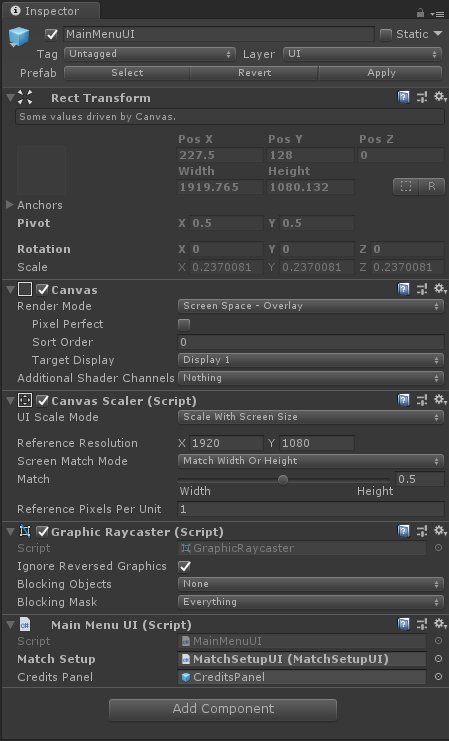
\includegraphics[scale=0.75]{\ImgPath/rys/GOMainMenuUI.png}
\end{center}
	\caption{Ekran inspektora po wybraniu obiektu MainMenuUI}
	\label{GOMainMenuUI}
\end{figure}

Dzieci obiektu MainMenuUI są już elementami samego UI. W ich skład wchodzą między innymi obiekty Grass, Basket oraz Logo, które są prostymi obrazkami. Posiadają jedynie komponenty typu RectTransform oraz Image. RectTransform odpowiada za pozycje obiektu na prostokątnym Canvasie. Komponent Image wyświetla teksturę na obszarze ograniczonym rozmiarem obiektu ustawionym w RectTransform. Tryb wyświetlania tekstury ustawiony jest na prosty - jest to statyczny obraz który nie zmienia się przez cały czas jaki jest wyświetlany. Kolejnym elementem jest animacja światła pod logiem. Jest to taki sam prosty obrazek jak poprzednie z tym że posiada dodatkowy komponent typu Animation. Odpowiada on za realizowanie prostych animacji. w tym przypadku jest to prosty obrót obrazka o 90 stopni w zapętleniu. Ponieważ obrazek jest symetryczny uzyskujemy efekt nieskończonego obrotu obrazka.

Dwa ostatnie dzieci to panele zawierające kolejne elementy UI. Panele pozwalają na łatwiejszą organizacje interfejsu użytkownika. Dzięki nim prościej jest też zrealizować np proste okno. Technicznie są to po prostu puste obiekty zawierające odpowiednio skonfigurowany komponent RectTransform oraz komponent typu Image. Pierwszy prostszy panel nazwany "CreditsPanel" jest oknem w którym znajdują się informacje o twórcach gry. Domyślnie jest on nieaktywny. zawiera obiekt który realizuje tekst poprzez komponent typu Text. Komponent ten zawiera pola takie jak: Text:, Font, Font Size, Alignment czy Color. W polu Text wpisywany jest tekst który jest wyświetlany na ekranie. To właśnie tutaj wpisane zostały informacje o twórcach. Font Size odpowiada za rozmiar czcionki. Tutaj wartość wynosi 63 ale zależna jest ona od tego ile tekstu jest wyświetlane - za duży rozmiar czcionki sprawi że tekst się nie zmieści. Font jest referencja do pliku zawierającego czcionkę którą renderowany jest tekst. Alignment odpowiada za to wyrównanie tekstu. W tym przypadku tekst jest wyśrodkowany zarówno w poziomie jak i w pionie. Ponadto panel ten zawiera jeszcze guzik który pozwala na zamknięcie okna. Jest on realizowany przez obiekt zawierający komponenty typu Button oraz Image. Komponent Button reaguje na eventy związane ze wskaźnikiem myszy. Wartość translation czyli przejście jest ustawione na Color Tint - zmiana koloru. Zależenie od tego czy przycisk jest w stanie domyślnym, znajduje się na nim myszka, jest kliknięty lub wyłączony zmienia się kolor obrazka ustawionego w komponencie Image. Pole On Click () odpowiada za przypisanie akcji które dzieją się po kliknięciu guzika. W tym przypadku podpięta jest jedna z funkcji skryptu MainMenuUI z głównego obiektu "MainMenuUI".

\begin{figure}[H]
	\begin{center}
\centering
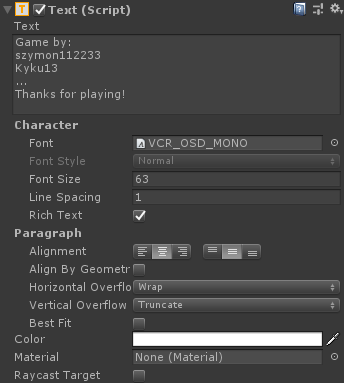
\includegraphics[scale=0.7]{\ImgPath/rys/text_component.png}
\end{center}
	\caption{Komponent Text}
	\label{text_component}
\end{figure}


\begin{figure}[H]
	\begin{center}
\centering
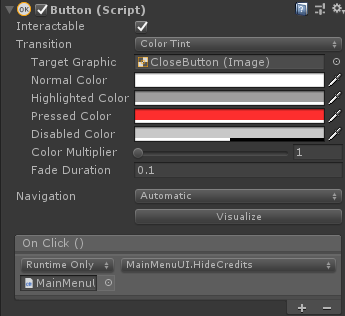
\includegraphics[scale=0.7]{\ImgPath/rys/button_component.png}
\end{center}
	\caption{Komponent Button}
	\label{button_component}
\end{figure}

Panel ButtonsPanel zawiera zestaw guzików do nawigacji w grze. Wszystkie z nich są niemalże identyczne. Różnią się tylko pozycja, tekstem oraz podpiętymi funkcjami. Sam panel zawiera dodatkowo komponent vertical Layout Group. Jest on odpoweidzialny za automatyczne równie ustawienie elementów UI w pionie. Komponent jest tak ustawiony że elementy wyrównane są do środka panelu. Pierwszy Guzik - Local Match - służy do rozegrania meczu na 2 graczy na komputerze lokalnym. Guzik Online Match przenosi nas do oddzielnego menu w którym znajdujemy partnera do gry meczu 2 osobowego online. Przycisk Credits otwiera wcześniej opisany CreditsPanel. Ostatni z przycisków - Exit, zamyka grę. Wszystkie guziki wykorzystują metody znajdujące się w skrypcie MainMenuUI.

Jednym z ważniejszych elementów sceny jest obiekt GameState. Zawiera on dane które muszą być dostępne w każdym skrypcie, dlatego też skrypt przypięty do niego zrealizowany jest jako singleton. Singleton w Unity realizowany jest poprzez stworzenie statycznej referencji do konkretnego obiektu. Obiekt takiej klasy podczas tworzenia sprawdza czy globalna instancja istnieje i jeżeli nie referencja zaczyna wskazywać na niego. W przeciwnym wypadku nowy obiekt jest od razu niszczony. Sam skrypt GameState jest głównie konternerem na dane i ma bardzo mało funkcji. Dane które przechowuje ten skrypt to:
\begin{itemize}
    \item isMultiplayer - prosta flaga mówiąca  o tym czy aplikacja działa w trybie online czy nie. Wiele funkcji w logice rozgrywki często sprawdza tą flagę żeby wiedzieć jak realizować swoje zdania.
    \item defaultGameData - referencja do instancji Scriptable Objectu typu GameDefaultData. Przechowuje on wartości domyślne ustawień meczu, dostępne w grze warianty kolorystyczne piłki i graczy, a także listę map. Obiekty typu Scriptable Object w odróżnieniu do Mono Behaviourów nie są instancjonowanie na scenie gry a w plikach na dysku. Instancja GameDefaultData znajduje się w projekcie gry a jej zawartość można zobaczyć na rysunku  \ref{default_game_data_instance}. Obiekt ten służy wyłącznie do odczytu i nie jest modyfikowany podczas gry.
    \item currentMatchSetup - obecne ustawienia meczu. Podczas inicjalizacji obiektu są one kopiowane z defaultGameData. Potem podczas gry gracz może je zmieniać poprzez okno ustawień meczu. Zawierają informacje o długości meczu, wybranej mapie, wariancie kolorystycznym piłki oraz graczy, ilości graczy oraz czasie odliczania przed meczem. Ostatnia wartość nie jest dostępna dla graczy, służy głównie do synchronizacji czasu w meczu online.
\end{itemize}

\begin{figure}[H]
	\begin{center}
\centering
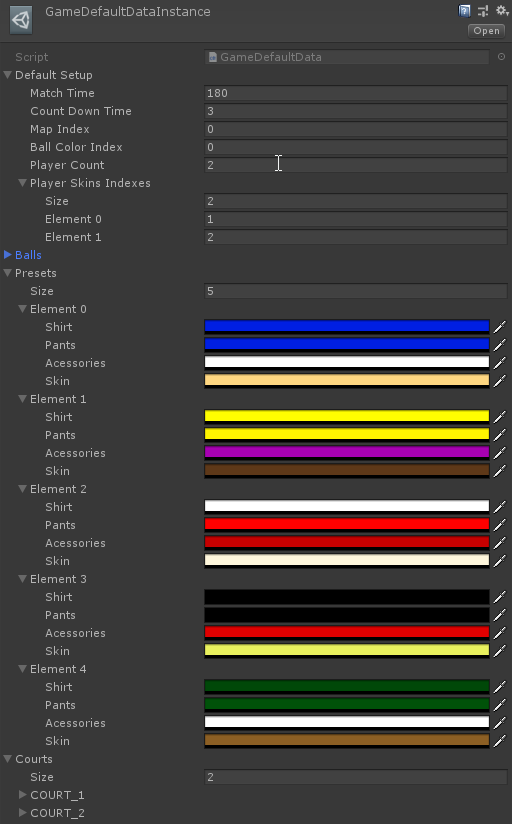
\includegraphics[width = 0.9\textwidth]{\ImgPath/rys/default_game_data_instance.png}
\end{center}
	\caption{Instancja GameDefaultData w grze}
	\label{default_game_data_instance}
\end{figure}

Na scenie znajduje się również obiekt MatchSetupUI. Odpowiada on za okno ustawień meczu - rysunek \ref{match_setup}. Obiekt ten  jest domyślnie ukryty i pojawia się dopiero gdy użytkownik będzie chciał uruchomić mecz. Okno używane jest zarówno w trybie lokalnym jak i online dlatego właśnie obiekt jest prefabem. Znajduje się również na scenie MultiplayerJoin. Z tych powodów obiekt posiada też oddzielne canvas - bez względu gdzie się znajduje, będzie działać niezależnie od reszty obiektów na scenie. W składzie okna znajdują się:
\begin{itemize}
    \item Wybór czasu meczu,
    \item Wybór wariantu piłki,
    \item Wybór mapy
    \item Wybór wariantów kolorów postaci graczy,
    \item Guziki: CANCEL oraz READY.
\end{itemize}
Każdy z elementów sterujących wyborem zawiera strzałki do zmiany aktualnie wybranej pozycji. Kliknięcie przycisku READY oznacza że akceptujemy ustawienia meczu i chcemy zacząć już rozgrywkę. Guzik CANCEL wyłącza okno i pozwala wrócić do głównego menu.

\begin{figure}[H]
	\begin{center}
\centering
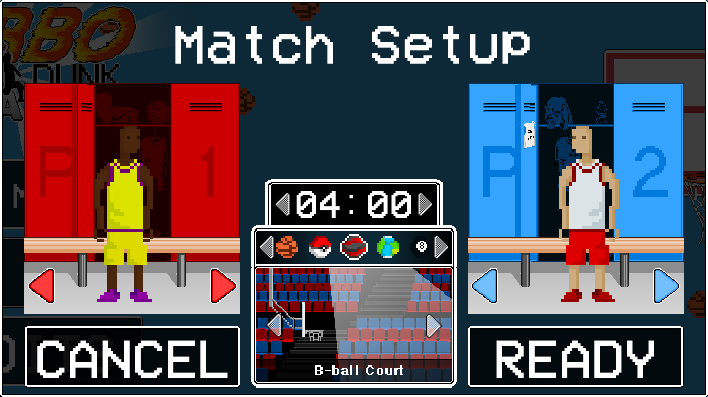
\includegraphics[width = \textwidth]{\ImgPath/rys/match_setup.png}
\end{center}
	\caption{Okno ustawień meczu}
	\label{match_setup}
\end{figure}

% Coś o spawnerze piłek

% Ustawinia kamery

Kolejną sceną w grze jest scena o nazwie "MutiplayerJoin". Znajduje się w niej głównie UI oraz inne obiekty związane z łączeniem się przez sieć z innym graczem. Scena jest wczytywana po wybraniu guzika Online Match w menu głównym. Funkcjonalność zostanie sceny zostanie szczegółowiej opisana w podrozdziale \ref{implementation_online}.

Ostatnie 2 sceny w grze są dość podobne - obydwie służą do samej rozgrywki. Różnią się głównie wyglądem tła oraz koszów. Mają też nieco zmienione Collidery. Na potrzeby tej pracy opisana zostanie tylko pierwsza z nich - COURT\_1. Scena opisywana będzie chwilę po rozpoczęciu gry, gdyż dopiero wtedy wszystkie niezbędone obiekty się na niej znajdują. W domyślnym widoku nie ma np. postaci graczy ponieważ są oni tworzeni dynamicznie na podstawie ustawień meczu. Lista ważniejszych elementów sceny:
\begin{itemize}
    \item Universe Manager - Główny obiekt decydujący o rozgrywce. W nim dzieję się niemalże cała logika meczu. Opisany bardziej szczegółowo poniżej w podsekcji \ref{universe_manager}.
    \item SceneRoot - Korzeń całej grafiki która znajduje się na planszy. Jego funkcja jest głownie organizacyjna ale pozwala też na manipulowanie całą planszą.
    \item GameplayUI - Obiekt zawierający komponent Canvas. Zajmuje się całą logiką z w interfejsem użytkonika wyświetlanym podczas meczu. Opisany bardziej szczegółowo poniżej w podsekcji \ref{gameplayui}.
    \item GameInput - Obiekt realizujący obsługę wejść w grze. Opisany bardziej szczegółowo poniżej w podsekcji \ref{gameinput}.
    \item MainCamera - Kamera główna renderująca całą scenę. Jej właściwości są sterowane obiektem komponentem Cinemachine Brain oraz obiektem VirtualCamera.
    \item VirtualCamera - Obiekt reprezentujący ustawienia kamery w module Cinemachine. Śledzi ona obiekt TargetGroup. Opisany bardziej szczegółowo poniżej w podsekcji \ref{virtualcamera}.
    \item TargetGroup - Pozycją tego obiektu jest uśredniony punkt wszystkich obiektów które śledzi kamera.
    \item Basket - Obiekt reprezentujący kosz. Posiada obręcz oraz punkt w który należy trafić żeby zdobyć punkty. Opisany bardziej szczegółowo poniżej w podsekcji \ref{basket}.
    \item GameState - Obiekt przechowujący stan gry. Jest przenoszony między scenami. Opisany bardziej szczegółowo wyżej.
    \item Player - Reprezentacja postaci sterowanej przez gracza w świecie gry. Opisany bardziej szczegółowo poniżej w podsekcji \ref{player}.
    \item Ball - Obiekt odpowiedzialny za fizyczną symulację piłki w dwóch wymiarach. Opisany bardziej szczegółowo poniżej w podsekcji \ref{ball}.
    \item Spawners - Zestaw obiektów reprezentujących pozycję początkową piłki oraz graczy. Są to zwykłe obiektu posiadające jedynie komponent typu Transform. Pozwalają na łatwe i wygodne ustawienie tych pozycji na scenie.
    \item Background - Zestaw obiektów posiadających komponent Sprite Renderer do stworzenia grafiki boiska. W jej skład wchodzi każdy element graficzny poza koszami, postaciami graczy piłką i interfejsem użytkownika.
    \item Platforms - Zestaw obiektów posiadających komponent Box Collider 2D reprezentujących fizyczne granice do poruszania dla postaci gracza. Aktualnie jest to jeden duży Collider służący jako podłoże do chodzenia oraz dwa Collidery pełniące rolę ścian blokujących graczy przed wyjściem poza planszę.
    \item BallOutColliders - Zestaw dwóch obiektów posiadających komponent Box Collider 2D, odpowiednie po lewej i prawej stronie poza strefą rozgrywki. Służą do wykrywania sytuacji gdy piłka zostanie wyrzucona poza boisko.
\end{itemize}

\begin{figure}[H]
	\begin{center}
\centering
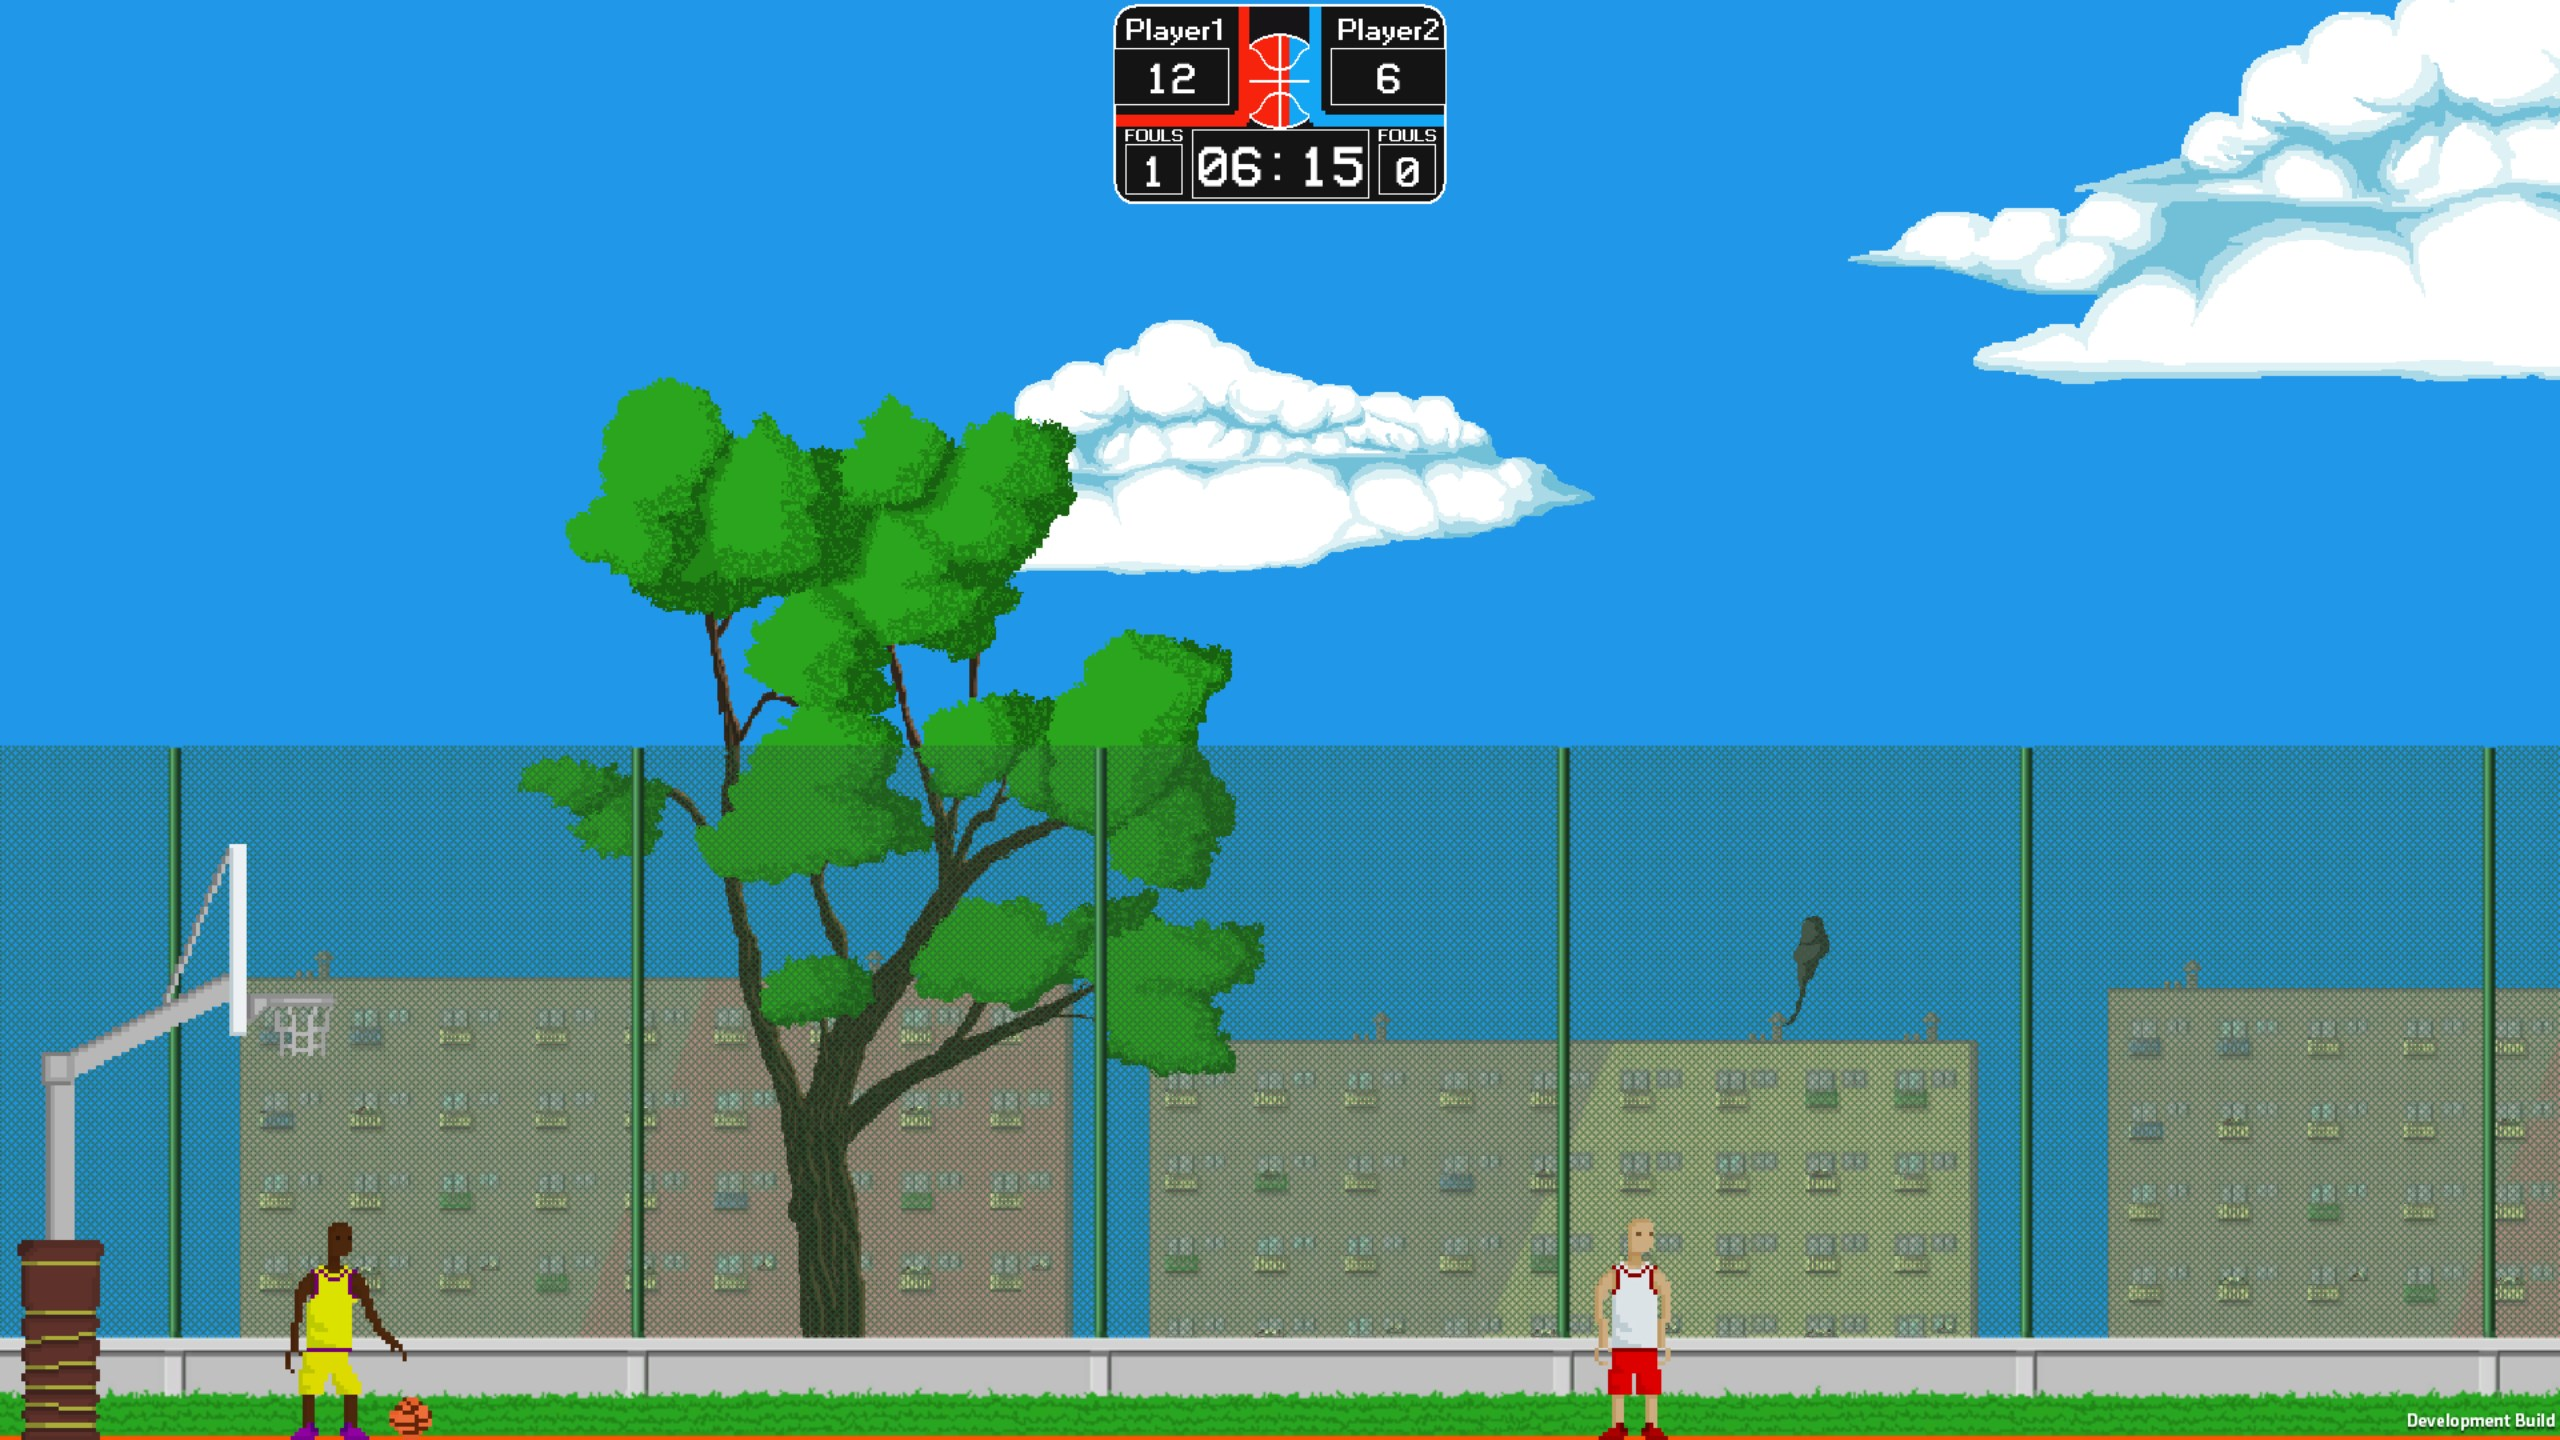
\includegraphics[width = \textwidth]{\ImgPath/rys/COURT_1.png}
\end{center}
	\caption{Scena COURT\_1 podczas rozgrywki}
	\label{COURT_1}
\end{figure}

\subsection{Universe Manager}
\label{universe_manager}
Obiekt zarządzający całą rozgrywką. Istnieje tylko jeden na scenie. jest realizowany jako singleton z tą różnicą że istnieje tylko na scenach z rozgrywką. Po opuszczeniu takiej sceny zostaje zniszczony i przy rozpoczęciu nowego meczu tworzony jest nowy obiekt. Jedynym komponentem tego obiektu jest skrypt UniverseManager który odpowiada za wspomniane właśnie funkcje. Kod wybranych funkcji można znaleźć w załączniku \ref{code_UniverseManager}. Implementacje funkcji różnią się zależnie od tego czy gramy w trybie online czy local.

Podstawą skrytpu jest zestaw funkcji czysto rozgrywkowych. Każda z ważniejszych mechanik w grze jest realizowana przez ten obiekt. Są to akcje takie jak: rzut piłki, wybicie piłki innemu graczu, popełnienie faulu oraz podnoszenie piłki. Działa to w taki sposób że gracz robiąc konkretne akcje uruchamia funkcje w skrypcie. W przypadku rzutu piłki gracz uruchamia funkcję SpawnBall() która za argument przyjmuje pozycje z której zostanie wyrzucona piłka, siłę rzutu oraz początkowy moment obrotowy piłki. Gracz po wywołaniu tej funkcji przyjmuje że piłka została wyrzucona, a sam skrypt zajmuje się już umieszczeniem piłki o danych parametrach w świecie gry. Wybicie piłki wygląda bardzo podobnie do wyrzutu. Informuje ona gracza który został uderzony że nie stracił on piłkę, wykonując na nim funkcję GetHit(). Gracz w tej funkcji dostosowuje swój wewnętrzny stan do tej sytuacji i woła funkcję SpawnBall() na skrypcie. Podniesienie piłki przez gracza odbywa się poprzez zawołanie funkcji RequestPickupBall(). W wersji lokalnej jest ona trywialna - informuje gracza o podniesieniu przez niego piłki oraz ustawia odpowiednie flagi na obiekcie piłki. Flagi te sprawiają że nie może być ona podniesiona przez innego gracza, oraz że obiekt piłki zostanie zniszczony pod koniec klatki. Funkcja odpowiedzialna za faule - DoneFoul() W wersji lokalnej zwiększa tylko licznik fauli.

Kolejnym ważnym zdaniem skryptu jest monitorowanie stanu rozgrywki. Istnieją funkcje odpowiedzialne za początek i koniec meczu, zmianę liczników punktów oraz fauli a także obsługę wyrzucenia piłki poza obszar rozgrywki. Reszta obiektów na scenie jest informowana poprzez tzw. eventy czyli zdarzenia pod które dowolny obiekt może doczepić wykonanie własnej funkcji. Są one zaimplementowane używając C\# akcji (System.Action). Zdarzenia takie występują np. gdy mecz się zakończy lub zmieniony zostanie wynik. Skrypt ten też liczy czas rozgrywki i aktualizuje co klatkę pozostały czas meczu w sekundach.

\subsection{GameplayUI}
\label{gameplayui}
Obiekt odpowiedzialny za wizualizacje stanu meczu. Posiada komponent typu Canvas oraz skrypt GameplayUI. jego dziećmi są poszczególne elementy UI takie jak tekst czy grafiki. Wyświetla aktualne stany liczników punktów oraz fauli, a także pozostały czas do końca meczu. Wartości te są aktualizowane poprzez nasłuchiwanie na eventy skryptu UniverseManager. Dla przykładu po zdobyciu punktów wysyłany jest odpowiedzialne zdarzenie. Skrypt GameplayUI obsługuje te zdarzenie poprzez zmianę tekstu odpowiedzialnego za wyświetlanie punktów. Pod koniec meczu wyświetlany jest dodatkowo ekran podsumowujący mecz.

\subsection{Player}
\label{player}
Jest to obiekt o najbardziej skomplikowanej hierarchii, zawierający wiele obiektów jako dzieci. Są to głównie obiekty zawierające komponenty Box Collider 2D. Każdy Collider ma inny cel, zaczynając o głównego Collidera który definiuje fizyczne granice obiektu, kończąc na wykrywaczu piłki. Najważniejszy jest jednak skrypt o nazwie TSDUPlayer znajdujący się na głównym obiekcie. Odpowiada on za poruszanie postacią gracza oraz wykonywanie akcji. W samym skrypcie znajduje się zarówno logika i zestaw zmiennych od których zależna jest ta logika. Przykładami zmiennych może być szybkość poruszania się czy siła wyskoku.

Dzieckiem tego obiektu jest również obiekt zawierający komponenty Sprite oraz Animator. Jest to reprezentacja graficzna postaci gracza. Zawiera ona liczne animacje poklatkowe. Animacje te są sterowane za pomocą maszyny stanów. Przejścia między stanami determinowane są poprzez zmiany flag w maszynie stanów. Za miane flag odpowiada również skrypt TSDUPlayer. Na rysunku \ref{anim_state_machine} pokazany jest schemat maszyny stanów. 

Kolejnym ciekawszym dzieckiem jest obiekt odpowiedzialny za wyświetlanie wskaźnika siły rzutu. Pojawia się on tylko gdy przycisk rzutu jest wciśnięty. Jest kontrolowany również przez skrypt TSDUPlayer na głównym obiekcie. Sam obiekt posiada komponent Canvas którego tryb wyświetlania ustawiony jest na przestrzeń trójwymiarową. Dzięki temu możemy korzystać z wszystkich elementów interfejsu użytkownika.Jedna z funkcjonalności komponentu Image, jest tutaj bardzo przydatna 0 zmiana typu obrazu. Typ obrazu ustawiony na został na Fill, a tryb wypełniania na pionowy. Poprzez miane wartości pola fill ammount uzyskujemy w bardzo prosty sposób pasek wskazujący aktualną siłę rzutu. Gdy fill ammount wynosi 1 widoczny jest cały obrazek i oznacza to maksymalną siłę rzutu. W przeciwnym wypadku (fill ammount = 0) obrazek jest niewidoczny i oznacza on minimalną siłę.  

\begin{figure}[H]
	\begin{center}
\centering
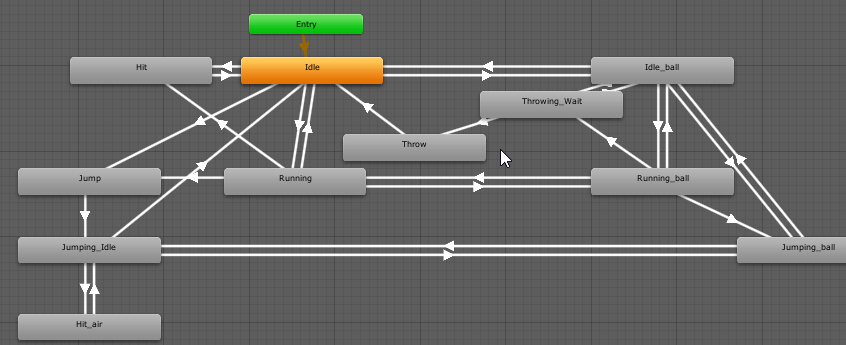
\includegraphics[width = 1.45\textwidth, angle = -90]{\ImgPath/rys/anim_state_machine.png}
\end{center}
	\caption{Maszyna stanów animatora postaci gracza}
	\label{anim_state_machine}
\end{figure}

\subsection{Ball}
\label{ball}
Bardzo prosty obiekt reprezentujący piłkę. Zawiera takie komponenty jak Sphere Collider 2D, Rigidbody 2D, Sprite Renderer oraz skrypt BallCollisionDetector. Wartości Rigidbody są ustawione tak żeby realnie oddać fizyczne zachowanie piłki w dwóch wymiarach. Jej ustawienia można zaobserwować na rysunku \ref{rigidbody_ball}. Collider odpowiada wielkością spritowi piłki. Skrypt odpowiedzialny jest za informowanie UniverseManagera o zderzeniach, lub wyleceniu poza boisko, w przypadku gdy czas gry dobiegł końca. Gra kończy się dopiero wtedy, pozwala to na decydujące rzuty w ostatnich sekundach trwania meczu.

\begin{figure}[H]
	\begin{center}
\centering
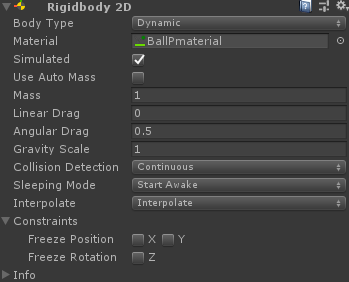
\includegraphics[width = 0.7\textwidth]{\ImgPath/rys/rigidbody_ball.png}
\end{center}
	\caption{Komponent Rigidbody 2D na obiekcie Ball}
	\label{rigidbody_ball}
\end{figure}

\subsection{Basket}
\label{basket}

Obiekt ten jest reprezentacją graficzną kosza do którego należy wrzucić piłkę aby zdobyć punkty. Na ten obiekt składa się kilka mniejszych obiektów zawierających komponenty Collider. Dzięki temu łatwiej jest odwzorować skomplikowany kształt kosza, co daje satysfakcjonujące efekty dobić piłki. Sama obręcz kosza posiada na jej dole specjalny obiekt który poza zwykłym Colliderem posiada też komponent Platform Effector 2D który pozwala piłkom na przenikanie przez niego z góry ale blokuje piłki lecące od dołu. Dzięki temu nie możliwe jest wrzucenie piłki do kosza o dołu. Ponadto, w środku siatki kosza znajduje się mały Collider wykrywający piłkę. Jeżeli piłka go dotknie, naliczany jest punkt.

\subsection{GameInput}
\label{gameinput}
Obiekt ten zawiera, poza Transformem tylko jeden komponent - skrypt GameInput. Jest on odpowiedzialny za sczytywanie stanu urządzeń wejść. Obiekt ten jest singletonem. Posiada metody zwracające boola z zapytaniem o to czy dany guzik jest kliknięty, został właśnie kliknięty lub został właśnie puszczony. Parametrami tych funkcji jest numer gracza oraz kod klawisza o który pytamy. Posiada również podobne metody zwracające wartości osi. Osie są metodą na dokładniejsze dostarczanie stanu wejść do software. Dla przykładu, gałki pada do gry posiadają 2 osie - pionową i poziomą, reprezentujące kierunek wychylenia gałki. Osie te mają wartość w przedziale <-1 ; 1>. Kiedy wychylimy gałkę maksymalnie do przodu wartość osi pionowej wynosi 1 a poziomej 0. W przypadku klawiatury kliknięcie przycisku prawej strzałki oś pozioma wskazuje wartość 0. Argumentami tych funkcji są numer gracza oraz nazwa osi. 

\subsection{VirtualCamera}
\label{virtualcamera}
Obiekt zawierający skrypt Cinemachine Virtual Camera z modułu Cinemachine. Jest to bardzo  zaawansowany skrypt posiadający wiele możliwości. Służy do zaawansowanej obsługi kamery, zarówno dwu jak i trójwymiarowej. Większość jej możliwości nie jest wykorzystywana w grze. Najważniejszą funkcja jest podążanie za obiektami. Kamera przesuwa się tak żeby w kadrze były wszystkie obserwowane elementy. Jeżeli nie jest możliwe objęcie wszystkich w jednym kadrze powiększa się on aż do momentu w którym spełniony jest ten warunek lub maksymalny rozmiar zostanie osiągnięty. 

\subsection{TargetGroup}
\label{targetgroup}
Obiekt zawierający skrypt TargetGroup z modułu Cinemachine. Skrypt ten wyznacza średnie centrum listy Transformów podanych jako target. Sam obiekt znajduje się zawsze w tym centrum. W ten sposób kamera śledząca ten punkt zawsze obejmuje na wszystkie obiekty w grupie. Dodatkowo możliwa jest ustawienie ciężkości każdego z Transformów tak żeby środek był przesunięty bardziej w stronę cięższych Transformów, oraz zmiana promienia, tak żeby nie tylko pojedynczy punkt - pozycja Transformu znajdowała się w kadrze, a większa obszar wyznaczony okręgiem o danym promieniu, gdzie sam Transform jest środkiem.




\section{Implementacja trybu online multiplayer}
\label{implementation_online}
Tryb online multiplayer oznacza konieczność synchronizacji części stanu gry między dwoma jej instancjami. Unty posiada wbudowany moduł odpowiedzialny za komunikację online ale nie jest on zbyt wydajny i posiada stosunkowo duży próg wejścia. Najlepszym pomysłem okazało się więc skorzystacie z rozwiązania które oferuje ExitGames. Jest to plugin do Unity o nazwie Photon. Jest to rozwiązanie które oferuje bardzo prostą synchronizację obiektów w Unity. Photon wykorzystuje architekturę klient-serwer. w chmurze zwaną Photon Cloud tworzone są serwery które zarządzają pokojami dla konkretnej gry. Instancje gry są klientami którzy dzielą się informacjami poprzez serwer. Żeby 2 graczy mogło wspólnie grać musi zostać nowiazne miedzy nimi połczenie. Nawiazywanie połaćzenia w Photonie polega na:
\begin{enumerate}
    \item Połączenie klienta z name serwerem. Jest na nim ustalany region z którym klient ma najszybsze połączenie.
    \item Połączenie klienta z master serwerem danego regionu. Master serwer posiada informacje o wszystkich serwerach gier które aktualnie działają w chmurze. Klient jest przekierowywany na serwer gry w która aktualnie gra.
    \item Połączenie z game serwerem. Game serwer zawiera listę lobby gry w której znajdują się pokoje dla danej gry.
    \item Klient łączy się z wybranym pokojem na wcześniej ustalonych zasadach. po dołączeniu do pokoju możliwy jest swobodny przepływ informacji między klientami.
\end{enumerate}

\begin{figure}[H]
	\begin{center}
\centering
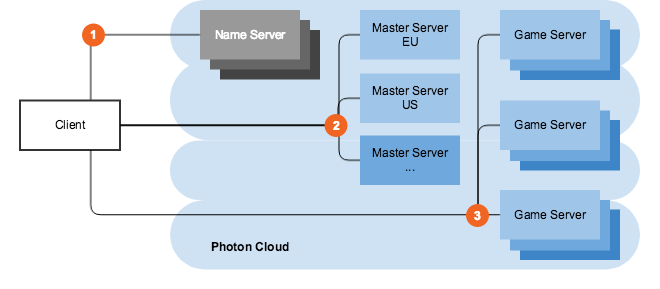
\includegraphics[width = 0.9\textwidth]{\ImgPath/rys/photon_cloud_structure.png}
\end{center}
	\caption{Struktura chmury Photon Cloud}
	\label{photon_cloud_structure}
\end{figure}

Wybór pokoju jest zależny od tego jaki opcje wybrał wcześniej gracz. Wybór tych opcji jest zrealizowany poprzez scenę MultiplayerJoin. Scena ta zawiera jedynie obiekty interfejsu użytkownika i służy do połączenia 2 graczy  oraz wybrania ustawień meczu. Możliwe są  typy rozgrywki online:
\begin{itemize}
    \item Random - Dołączenie do losowego pokoju. Po kilknięciu tego guzika rozpoczyna się proces połączenia z serwerem oraz dołączania do pokoju. Jeżeli żaden pokój nie istnieje lub wszystkie są zajęte tworzony jest nowy pokój.
    \item Friends - Dołączenie do pokoju ze znajomym. Wybranie tej opcji otwiera menu wpisywania sekretnej frazy. Znajdują się też tam informacje tłumaczące działanie gry ze znajomymi. Po wpisaniu frazy rozpoczyna się proces łączenia z serwerem oraz tworzenia pokoju. Nazwą tworzonego pokoju jest sekretna fraza, oraz jest on niedołączalny poprzez losowy wybór pokoju. Jeżeli istnieje już pokój o takiej nazwie klient dołącza do niego. W ten sposób znajomi wpisując taką samą sekretną frazę upewniają się że grają ze sobą. Jeżeli istnieje już pełen pokój o takiej nazwie nie zostanie on stworzony a gracz zostanie poinformowany o konieczności zmiany sekretnej frazy.
\end{itemize}

Po stworzeniu pokoju klient czeka na dołączenie gracza do pary. Po dołączeniu obydwu graczy wysyłana jest informacja do obu klientów o rozpoczęciu wyboru ustawień meczu. Klient który założył serwer jest tzw. master klientem. Pozwala mu to na decydowanie o nieścisłościach podczas meczu oraz wybór większości ustawień meczu. Wybór ustawień wygląda podobnie do Wyboru podczas trybu lokalnego, z tą różnicą że guzik READY wysyła informację o gotowości do drugiego klienta. zmiany wyborów ustawień wysyłane są też do drugiego klienta dzięki czemu są one u niego widoczne.

Po tym jak każdy z graczy jest w trybie gotowości, następuję rozpoczęcie meczu. Master klient wysyła informacje o konieczności załadowania konkretnej mapy do drugiego klienta. Po załadowaniu mapy master klient czeka na informacje od drugiego klienta o poprawnym załadowaniu poziomu. Po otrzymaniu tej informacji, wysyłane są jako odpowiedź informacje o zestawie ustawień meczu o raz planowanym czasie jego rozpoczęcia. Master klient zajmuje się załadowaniem sterowanych przez niego obiektów, po czym rozpoczyna odliczanie do startu meczu. Drugi klient po otrzymaniu informacji z ustawieniami meczu, dostosowuje lokalne ustawienia do tych otrzymanych, ładuje sterowane przez niego obiekty oraz ustawia czas odliczania tak aby start meczu był zsynchronizowany na obu maszynach. Po zakończeniu meczu master klient wysyła policzony wynik podsumowania meczu do drugiego klienta. Następnie na obu klientach wyświetlane jest okno z podsumowaniem meczu.

Synchronizacja rozgrywki odbywa się poprzez dołączenie do obiektów synchronizowanych odpowiednich komponentów dostarczonych przez Photona. Do każdego obiektu typu Player dodany został komponent typu PhotonView. Zajmuje się on synchronizacją komponentów sieciowych. W przypadku tego obiektu jest to komponent typu PhotonAnimatorView oraz skrypt TSDUPlayer który został rozszerzony o możliwości sieciowe. Komponent PhotonAnimatorView służy do synchronizacji flag animatora. dzięki temu na obu maszynach wykonywane są te same animacje. Skrypt TSDUPlayer odpowiedzialny jest za synchronizację pozycji oraz rotacji postaci gracza. W skrypcie tym została również zaimplementowanie tak zwane lag compensation. Polega to na tym że obiekt jest przesuwany na podstawie ostatniej informacji jaka została otrzymana. Jeżeli np. otrzymana została informacja o pozycji obiektu, brane jest pod uwagę jego przesunięcie oraz czas w którym została wysłana ta informacja. Na podstawie tych danych obiekt przesuwany jest o dodatkową, obliczoną wartość. Dzięki temu obiekt przesuwa się nieco płynniej i nie jest widoczna jego teleportacja. 

Do obiektu typu Ball również został dodany skrypt typu PhotonView. Obserwuje on specjalnie stworzony skrypt o nazwie BallNetworkSync. Odpowiedzialny jest on za synchronizację piłki na obu maszynach. Wysyłana jest rotacja, pozycja oraz prędkość piłki. W wersji replikowanej piłki czyli kliencie który nie steruje piłką, fizyka piłki jest również liczona z tym że jej pozycja, rotacja i prędkość jest ciągle poprawiana poprzez dane dostarczone od klienta sterującego piłką. Dzięki temu piłka porusza się płynnie na obu maszynach. Dodatkowo zaimplementowane jest w tym skrypcie lag compensation.  

Reszta stanu meczu synchronizowana jest poprzez zdarzenia sieciowe. Działają one podobnie do zdarzeń zaimplementowanych za pomocą System.Action, z tą różnicą że zdarzenie wysyłane jest nie tylko do konkretnych obiektów ale przede wszystkim do konkretnych maszyn. W ten sposób właśnie zaimplementowane zostało uderzenie postaci gracza, rzut piłką czy zmiana wyniku. Kod przykładowego zdarzenia znajduje się w dodatku \ref{code_PhotonEventExample}. Zdarzenia zawierają też dane niezbędne do odtworzenia stanu gry na drugim urządzeniu. Są one bardzo wydajne, a także niezawodne. Nie ma wiec ryzyko że jakieś wydarzenie nie  zostanie dostarczone do klienta docelowego.




\section{Przygotowanie gry pod nowe platformy}
Zagadnienie tzw. portowania czyli przeniesienia gry na nową platformę, jest dość rozbudowane. Jak okazało się podczas procesu tworzenia gry, większość rzeczy jaki można zrobić to pisanie kodu który jest czysty, przejrzysty oraz łatwo skalowalny. Znacznie przyspiesza to ten proces i pozwala unikając błędów wynikających z niezrozumienia kodu. Wiele funkcjonalności które przynoszą zwykle problem podczas procesu przenoszenia nie zostało jeszcze zaimplementowanych lub po prostu nie jest planowane dodawanie ich. Można do nich zaliczyć takie rzeczy jak; system zapisów, tablice wyników czy osiągnięcia.

Jednym z głównych narzędzi używanych podczas portowania jest abstrakcja. Dobrym przykładem użycia abstrakcji do ułatwienia procesu portowania jest skrypt GameInput. Korzysta on ze zmiennych implementacji Metod GetButton, GetButtonPressed, GetButtonReleased, GetAxis w klasie InputPlayer. Kod tej klasy można znaleźć w dodatku \ref{code_InputPLayer} Tworzone są klasy dziedziczące po  klasie InputPlayer i przeciążają jej metody. W ten sposób może być realizowana obsługa różnych urządzeń wejścia. W przypadku komputera metody te zwracają wartość true/false lub wartość typu float w przypadku ostatniej metody, zależnie od stanu klawiszy na klawiaturze komputera. Argumentami funkcji są wartości enumów GameButtons i GameAxis. Dzięki takiemu rozwianiu skrypt GameInput zawsze pyta o klawisz odpowiedzialny za jakąś akcje, a nie konkretny przycisk na klawiaturze. Za ustawienie przycisków odpowiedzialnych za akcje odpowiada klasa dziedzicząca po klasie InputPlayer. Posiada ona po prostu zestaw pól w których zapisywane są kody fizycznych guzików. Dzięki zastosowaniu takiego rozwiązania możliwa jest łatwa zmiana przycisków odpowiedzialnych za akcje na danym urządzeniu wejścia. na obecny moment wartości te są ustawiane podczas inicjalizacji gry, jednak w przyszłości możliwe będzie ich zmiana podczas uruchomienia aplikacji.

Kolejnym ważnym aspektem podczas portowania jest wydajność na docelowym urządzeniu. Gra omawiania w niniejszej pracy nie jest wymagająca obliczeniowo. Największym problemem na konsolach o słabszych możliwościach może być jednak obliczanie fizyki oraz warstwa sieciowa. Jeżeli chodzi o fizykę - głównym powodem jej liczenia jest piłka. W menu głównym spadające piłki opierają się na fizyce, żeby spadać. Piłek jest dużo ale dzięki zastosowaniu tzw. object poolingu ich liczba jest kontrolowania a pojawienie się kolejnych piłek jest tylko kwestią aktywacji obiektu oraz zmiany jego położenia i prędkości. Object pooling polega na stworzeniu organicznej liczby obiektów danego typu oraz dezaktywacji ich. Kiedy w grze istnieje potrzeba stworzenia nowego obiektu, zamiast alokować pamięć, wykorzystany jest istniejący już w pamięci nieaktywny obiekt. Analogicznie zamiast usuwać obiekt którego już nie potrzebujemy jest on po prostu dezaktywowany. Jeżeli fizyka będzie liczyć się za długo na nowych platformach wystarczy zmniejszyć ilość piłek. Piłka używana podczas meczu nie jest zbyt skomplikowana. Jej Collider jest to po prostu kołem, czyli jeden z prostszych kształtów jeżeli chodzi o obliczanie kolizji.

Aspekt sieciowy został szczegółowo opisany w rozdziale \ref{implementation_online}. Ważniejszą jego częścią, jeżeli chodzi o optymalizacje, jest ilość danych przesyłanych między urządzeniami. Większość danych jest wysyłana poprzez pojedyncze zdarzenia sieciowe. Jest to np. informacja o zmianach ustawień meczu czy zdobyciu punktu. Liczba obiektów które muszą wysyłać dane w regularnych odstępach czasu jest ograniczona do minimum. Do tych obiektów zaliczana jest piłka oraz postacie graczy.

%-----------------
% Testowanie
%-----------------
\chapter{Przetestowanie opracowanej gry komputerowe}

Zagadnienie przetestowania całej gry komputerowej jest ogromnym zadaniem - ilość możliwych stanów jakich może znaleźć się aplikacja jest kolosalna. Wiele gier mimo uznania je za kompletne i wydania wersji 1.0 posiada liczne błędy. Zwykle im większa jest gra tym więcej zawiera błędów. Kluczową rzeczą jest upewnienie się nie że gra nie posiada błędów ale że nie posiada błędów które uniemożliwiają rozgrywkę lub sprawiają że staje się ona bardzo trudna albo nieprzyjemna. Dobrze też żeby gra działała płynnie na docelowym sprzęcie - komputerze osobistym, konsoli czy urządzeniu mobilnym. 

%Ważne, pameitaj że w poprzednim roku na techniki multimedialne robiłeś samasymulacje piłki - były to ponieka testy.

\section{Gameplay}

Najważniejszymi testami w przypadku gier są testy prowadzane przez użytkowników - w tym przypadku graczy. W celu przetestowania projektu został stworzony serwer na platformie Discord. Platforma ta pozwala na komunikację natychmiastową (zarówno tekstową jak i głosową) na licznych kanałach założonych przed administratora serwera. Na serwer została zaproszona grupa 20 osób której udostępnioną została najnowsza stabilna wersja gry. Dodatkowo zostały założone kanały tekstowe których celem było opisywanie błędów, dodawanie sugestii oraz ogólnie rozmowy o grze. Część błędów zgłoszonych do czasu powstania pracy została naprawiona, a część wciąż czeka na naprawę. Nie są to jednak rzeczy uniemożliwiające rozgrywkę dzięki czemu testerzy mogą dalej grać w grę i znajdować nowe błędy. Przeprowadzono również tzw. stress testy, czyli zachowanie aplikacji podczas dużego obciążenia. W przypadku gry, darmowy plan Photona pozwala na zaledwie 20 graczy, co wyznacza maksymalną ilość graczy grających na raz w grę w trybie online. W tym celu zostały założone też 3 dodatkowe kanały głosowe na serwerze Discord. Testerzy zebrali się 24 stycznia 2019 w godzinach wieczornych w celu przeprowadzenia tych właśnie testów. W ich wyniku zostało stwierdzone kilka nowych błędów podczas rozgrywki jednak sam system łączenia graczy w pary działał bardzo dobrze i nie udało się znaleźć żadnego błędu.

\section{Wydajność}
Wyżej wspomniani gracze korzystali z prywatnych komputerów i laptopów do testowania, w celu zbadania możliwych problemów z wydajnością. Do debugowania wydajności w grach bardzo często korzysta się z profilerów. Są to specjalne programy liczące czas wykonania każdej funkcji. Podczas testów żadnemu z testerów nie zdarzyły się problemy z wydajnością. na rysunkach poniżej zostały zamieszczone wyniki działania profilera podczas uruchomienia menu głównego (rysunek \ref{profiler_mainmenu}) oraz meczu (rysunek \ref{profiler_gameplay}). Tak jak jest to spodziewane gra działa bardzo płynnie. Nie jest ona skomplikowana obliczeniowo.

\begin{figure}[H]
	\begin{center}
\centering
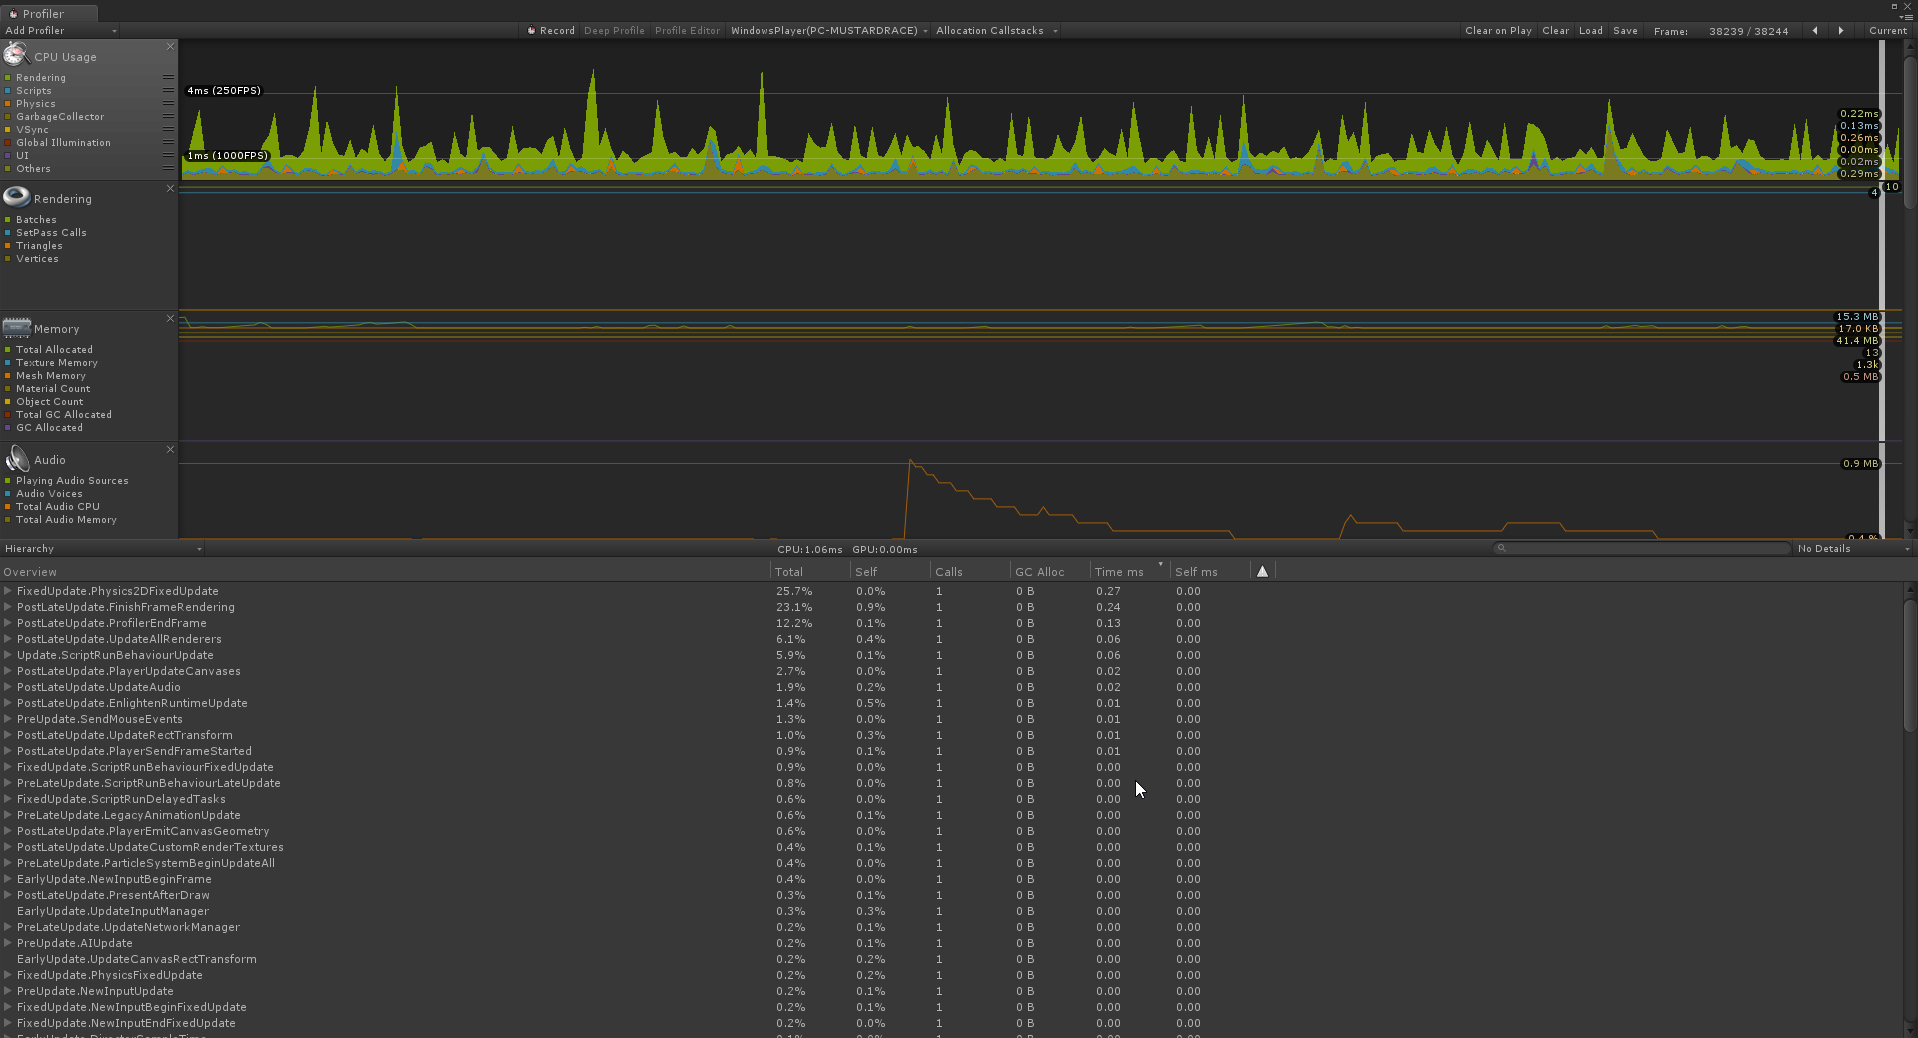
\includegraphics[width =\textwidth]{\ImgPath/rys/profiler_mainmenu.png}
\end{center}
	\caption{Okno profilera podczas działania gry w menu głównym}
	\label{profiler_mainmenu}
\end{figure}

\begin{figure}[H]
	\begin{center}
\centering
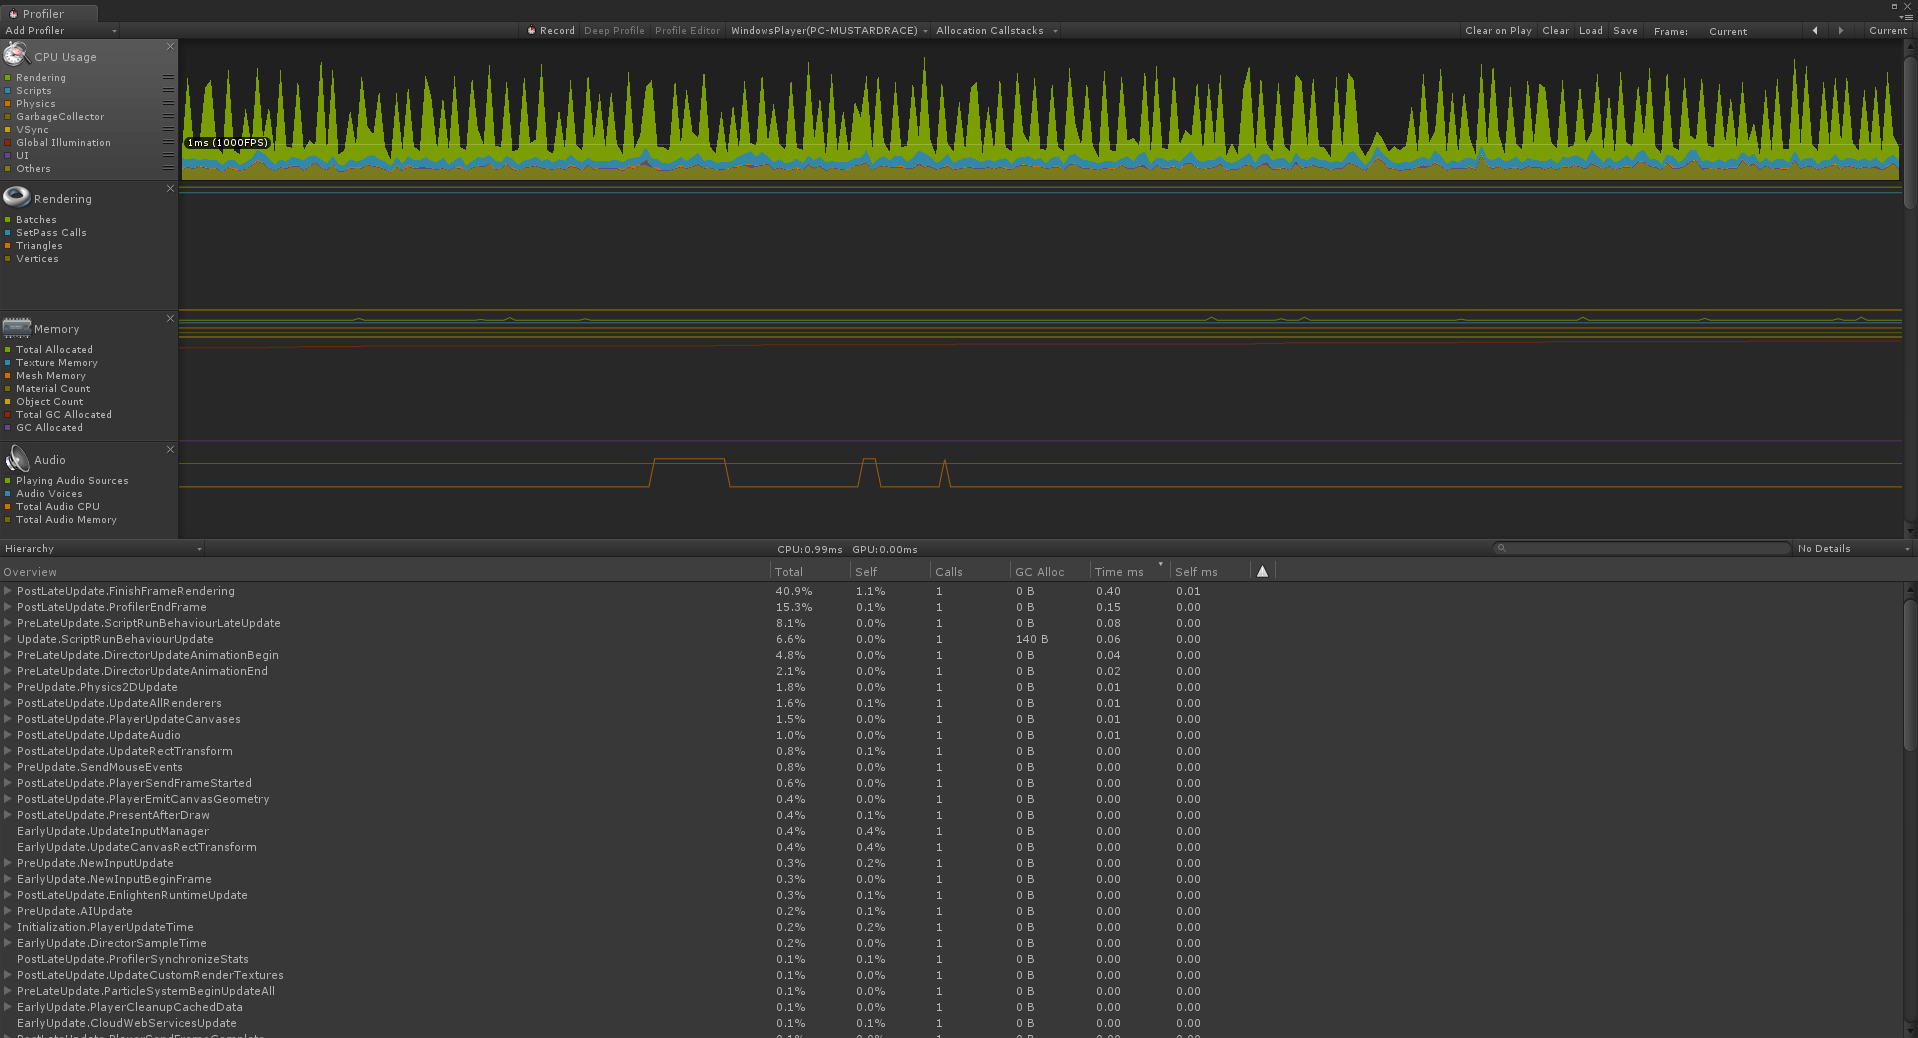
\includegraphics[width = \textwidth]{\ImgPath/rys/profiler_gameplay.png}
\end{center}
	\caption{Okno profilera podczas działania gry w trakcie trwania meczu}
	\label{profiler_gameplay}
\end{figure}

%-----------------
% Podsumowanie i wnioski 
%-----------------
\chapter{Podsumowanie i wnioski }

%minimum 2 strony w tym opis problemow programistycznych i ich rozwiazanie, perspektywy rozwoju gry itp

\begin{thebibliography}{99}
\addcontentsline{toc}{chapter}{Bibliografia}
\bibitem{gamejolt_page}{Gra Turbo Slam Dunk Unleashed w serwise GameJolt. \url{https://gamejolt.com/games/turbo-slam-dunk-unleashed/123485} [dostęp 14 stycznia 2019]}
\bibitem{unity_wiki} {Strona Wikipedi poświęcona Unity  \url{https://en.wikipedia.org/wiki/Unity_(game_engine)} [dostęp 17 stycznia 2019]}
\bibitem{canalplus_gry} {Twórcy Światów - Dokument zrealizowany przez Canal + \url{https://www.canalplus.pl/discovery/tworcy-swiatow}}
\bibitem{wiki_gameshistory} {Historia gier komputerowych na Wikipedi: \url{https://pl.wikipedia.org/wiki/Historia_gier_komputerowych} [dostęp 19 stycznia 2019]}
\bibitem{about_mono} {Oficjalna strona Mono \url{https://www.mono-project.com/docs/about-mono/} [dostęp 20 stycznia 2019]}

\end{thebibliography}

\listoffigures
 
\listoftables

\appendix
\chapter{Załączniki}
    \definecolor{codegreen}{rgb}{0,0.5,0}
\definecolor{codegray}{rgb}{0.5,0.5,0.5}
\definecolor{codepurple}{rgb}{0.58,0,0.82}
\definecolor{backcolour}{rgb}{0.95,0.95,0.97}
\definecolor{bluekeywords}{rgb}{0,0,1}
\definecolor{redstrings}{rgb}{0.64,0.08,0.08}
 
\lstdefinestyle{mystyle}{
    morekeywords={partial, var, value, get, set, using, class, public},
    backgroundcolor=\color{backcolour},   
    commentstyle=\color{codegreen},
    keywordstyle=\color{bluekeywords},
    numberstyle=\tiny\color{codegray},
    stringstyle=\color{redstrings},
    breakatwhitespace=false,         
    breaklines=true,                 
    captionpos=b,                    
    keepspaces=true,                 
    numbers=left,                    
    numbersep=5pt,                  
    showspaces=false,                
    showstringspaces=false,
    showtabs=false,                  
    tabsize=2,
    language=csh,
    basicstyle=\footnotesize\ttfamily,
    numbersep=5pt,
    extendedchars=true,
    frame=b,
    xleftmargin=17pt,
    framexleftmargin=17pt,
    framexrightmargin=5pt,
    framexbottommargin=4pt,
    commentstyle=\color{green},
    morecomment=[l]{//}, %use comment-line-style!
    morecomment=[s]{/*}{*/}, %for multiline comments
}
 
\lstset{style=mystyle}

\section{Kod skryptu MainMenuUI.cs}
    \lstinputlisting[language={[Sharp]C}, caption={Kod skryptu MainMenuUI.cs}, label={code_MainMenuUI}]{\ImgPath/Code/MainMenuUI.cs}

%\zakonczenie  % wklejenie recenzji i opinii

\end{document}
%+++ END +++
